\chapter{Propagating the Uncertainty from Stereo Images to the Cost Volume}\label{chap:propagating}
\comloic{tu n'imagines pas le bonheur que je ressens à l'orée de ce chapitre 4 (puis 5), c'est comme sortir d'une forêt obscure, rentrer à la maison et retrouver des odeurs communes, comme si plus rien ne pouvait arriver qui nous surprenne, c'est retrouver la serrenite, l'impression d'être à l'heure} The previous chapter presented different methods for joining credal sets using a copula\commanue{Alors moi je tournerais la phrase au passif In the previous chapter, different methods for joining credal sets using a copula have been presented}. In this chapter, we will see how those results\comloic{et là c'est le moment où tu comprends qu'il y a une continuité entre la forêt obscure et la maison, comme si tu n'étais pas rentré tout seul de là bas} can be applied to propagate the uncertainty in a stereo matching example. More specifically, we will use possibility distributions from \Cref{chap:representation_of_uncertainty} as uncertainty models on the intensity values of epipolar images used in stereo matching. We will then propagate the uncertainty from those images to the cost volume using results from \Cref{sec:necessity_functions}. We will also show that propagating the uncertainty has the potential to improve the disparity map derived from the cost volume. This chapter takes up work and data already published \cite{malinowski_copulas_2022, malinowski_uncertainty_2023}.

It is important to note that in this disparity estimation problem, we only account for the uncertainty in our input image intensities, without considering the uncertainty in our cost function's ability to correctly identify the true disparity as its minimum. In other words, we do not account for the uncertainty arising from the difference between ``two patches are very similar'' and ``the pixels at the center of the patches are homologous''. We refer to \Cref{fig:adherence_window} and the discussion in \Cref{sec:stereo_matching} regarding the adherence problem for more details. We focus in this chapter on the propagation of uncertainty. We will thus consider a stereo matching pipeline with a simple cost function and no \acrshort{sgm} regularization. Indeed, propagating the uncertainty through a cost volume optimization is too complex and computationally expensive to be solved with this chapter's method. We will consider the different problem of uncertainty modelling with \acrshort{sgm} regularization in the following chapter, \Cref{chap:epistemic_uncertainty}. 

\section{Context and Hypotheses for Uncertainty Propagation }\label{sec:sources_of_uncertainty}
\subsection{Considered Stereo Matching Pipeline}
We consider the Sum of Absolute Differences (SAD) as our cost function, presented in \Cref{sec:cost_volume_computation}, and reminded here. Given patches $W_L\subset I_L$ and $W_R\subset I_R$ of the same shape with $n$ pixels (usually squares):
\begin{align}
    \SAD(W_L, W_R) = \sum_{(p_i, q_i)\in (W_L, W_R)}|I_L(p_i) - I_R(q_i)|\label{eq:SAD}
\end{align}
where $p_i$ and $q_i$ are pixels at the same position $i$ in their patch. For convenience purposes, we will refer to the Absolute Difference between two pixels as AD (when there is no sum involved). An illustration of windows from stereo images to compare is presented in \Cref{fig:Cones}, and an illustration of the AD between pixels and $\SAD$ cost function can be found in \Cref{fig:SAD}.

\begin{figure}[ht]
  \centering
  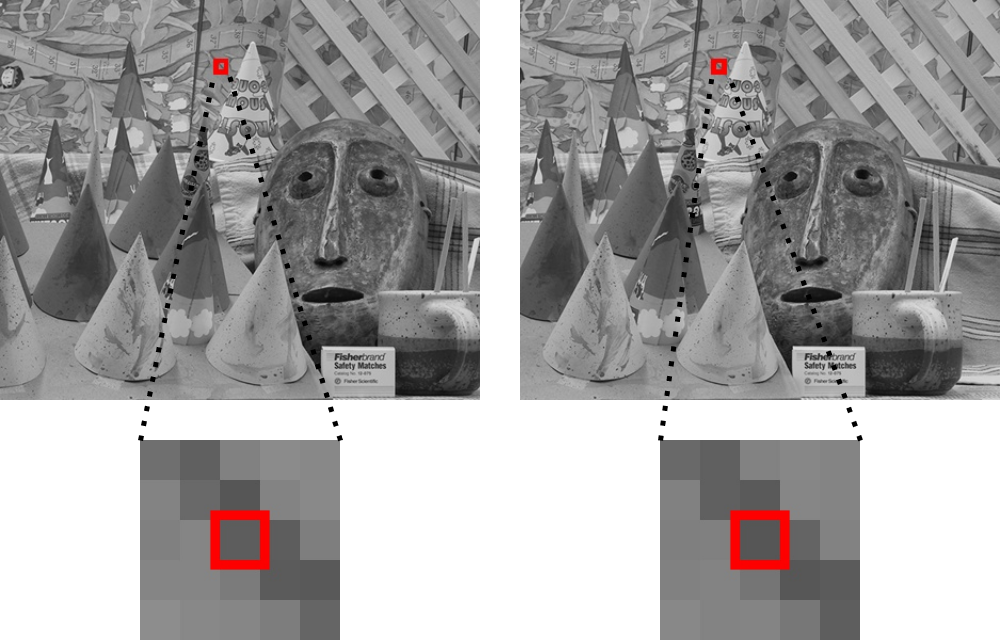
\includegraphics[width=0.8\linewidth]{Images/Chap_4/Cones.png}
  \caption{Homologous pixels in a pair of images. From \cite{malinowski_uncertainty_2024}}\label{fig:Cones}
\end{figure}

\begin{remark}
    Although the $\SAD$ is not the best performing cost function for dense matching, it is both fast and easily parallelizable. It is often use for comparison in cost-based stereo algorithms \cite{hirschmuller_evaluation_2007, zbontar_stereo_2016}, or in other applications. Considering a simple cost function such as $\SAD$ is relevant for different reasons:
    \begin{itemize}
        \item Simple stereo matching algorithms are often used as a quick and easy method for estimating the disparity.
        \item Simple cost functions (such as $\SAD$, ZNCC, \etc) considered here are still used in other problems, such as video compression for instance \cite{richardson_h264_2006}.
        \item As both stereo matching and uncertainty propagation can be complicated problems, considering a simple stereo algorithm allow us to remain (relatively) simple and didactic in our explanations. 
    \end{itemize}
\end{remark}

As stated previously, we will not consider in this chapter the use of Semi Global Matching (or similar regularization methods), as it necessitates many operations due to its recursive formulation and thus greatly increases complexity for the uncertainty propagation. We diverge from state-of-the-art methods to keep explanations as simple as possible, however the modeling of uncertainty for more advanced cost functions and \acrshort{sgm} methods will be considered in \Cref{chap:epistemic_uncertainty}.

\begin{figure}
    \centering
    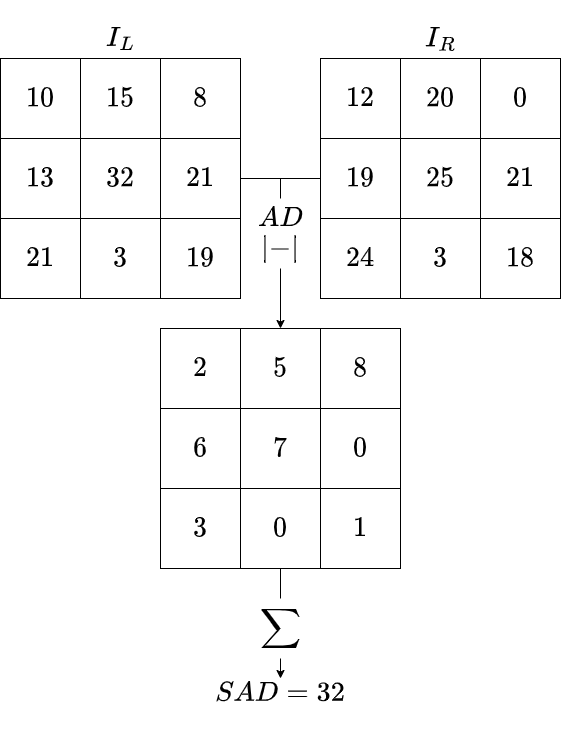
\includegraphics[width=0.5\linewidth]{Images/Chap_4/SAD.png}
    \caption{Diagram representing the $SAD$ cost function between two $3\times3$ patches. From \cite{malinowski_uncertainty_2024}}
    \label{fig:SAD}
\end{figure}

In our experiments, we considered the ``Cones'' images from the 2003 Middlebury stereo dataset (\url{https://vision.middlebury.edu/stereo/data/scenes2003/}), as presented in \Cref{fig:color_cones_image}. The two images have a of size $375 \times 450$, and the range of considered disparities is $[-60, 0]$.

\subsection{Uncertainty Model for Epipolar Images Intensities}
To maintain simplicity in this section, we will not consider panchromatic images, such as Pléiades products, encoding the reflectance values as positive integer, usually contained in $[0, 5000]$. Instead, we consider grayscale images that have intensity levels quantified within the range $[0, 255]$, which will represent our measurable space $\X$.

\begin{remark}
    This hypothesis is not constraining as we can easily normalize reflectances in order to encode them using 8-bit integers value, although doing so reduces the precision of the initial images. Moreover, this normalization step is often required to fit a given format, for instance if the images must be processed by a CNN trained on 8-bit integers.
\end{remark}

We hypothesize that a pixel's intensity value can deviate around its observed value with a range of $\pm i_\sigma$, with the observed value being the most likely. This specific hypothesis remains simple and relatively plausible with regards to the processing leading to the epipolar images. We then suppose that the uncertainty from the noise of the sensor capturing the image, from pre-processing steps such as atmospheric correction\commanue{alors cette étape je ne sais, après tu as tout de même des étapes de corrections radiométriques et géométriques} or epipolar resampling (see \Cref{sec:uncertainty_cars}) or from the quantification of observed radiometric values into integers\commanue{je ne suis pas sure de comprendre}, are not exactly known, but can be model by a possibility distribution. Consequently, we model the uncertainty of each pixel $p\in I_L,I_R$ intensity with a possibility distribution $\pi$, centered around the observed intensity $i_p\in[0,255]$:
\begin{equation}\label{eq:pixel_possibility}
    \pi(i_p)=1,\quad \pi(i_p\pm i_\sigma)=\alpha\,,
\end{equation}
with $\alpha \in [0,1]$. To remain simple, we chose $i_\sigma=1$ in the following, which is relatively narrow but allows simplification without impacting our reasoning. Similarly, we do not consider multiple $\alpha$ values in order to limit the number of focal sets considered. Choosing thus simple possibility distribution is convenient, but results obtained in this chapter can easily be extended to more complex possibility distributions. In our simulation, $\alpha = 0.3$ for pixels in the left image and $\alpha = 0.4$ for pixels in the right image\commanue{Je ne sais pas si tu synthétises les valeurs quelque part mais ce serait cool, ça peut être un tableau en annexe, sinon ça oblige à relire la section pour retrouver les valeurs}. We use different values of $\alpha$ for the left and right images because the uncertainty model may vary between images due to differences in exposure, noise levels, or camera calibration. The values on themselves are chosen arbitrarily for the purpose of this example. From a credal set interpretation, this model effectively states that we accept any probability distribution supported within $[i_p - 1, i_p + 1]$ where the probability measure $P$ satisfies $\{P(A) \leq \sup_{i \in A} \pi(i)\}$ as an acceptable model for our uncertainty. The mass distribution function $m_p$ associated to this credal set possesses two focal sets $a^p$:
\begin{eqnarray}
    &m_p(a^p_1=\opi i_p, i_p\cli)=1-\alpha\,\nonumber\\
    &m_p(a^p_2=\opi i_p-1, i_p + 1\cli)=\alpha\,\label{eq:pixel_mass}
\end{eqnarray}
with $\opi\cdot, \cdot\cli$ referring to integer intervals. In particular, $\opi i_p, i_p\cli$ correspond to the singleton $\{i_p\}$.

\begin{remark}
    The hypothesis of modelling the uncertainty on image intensities by possibility distributions does not consider uncertainty from potentially bigger sources of errors, such as satellite vibrations during the acquisition, or errors in the computations of epipolar lines. Those type of errors have been encountered on some Pléiades acquisitions, and lead to significant biases and errors on the final DSM, that our simple model does not account for. However, the CO3D mission will acquire images using a CCD matrix sensor rather than push-broom sensors used in Pléiades, so we can safely assume that those problems should not be encountered on images from the CO3D mission\commanue{Bon disons plutôt que la correction géométrique des images a pour objectifs de tenir compte de ces erreurs éventuelles et de les minimiser.}.
\end{remark}


\subsection{Dependency Model between Epipolar Images}
We presented the uncertainty models for pixels in both images, but we also need to define the dependency model between every pixel of both images. Indeed, as some pixels between images represent the light reflected by the same object, it seems natural that their (uncertain) values are correlated. In our case, we propose to model their dependency with the product copula if the pixels are not from the same physical object, meaning that the value of their intensities are independent. For pixels belonging to the same object, we model their dependency by a Gaussian copula with a covariance matrix $R$. Those copulas were presented in \cref{eq:gaussian_copula} from \Cref{chap:representation_of_uncertainty}. We remind here the formulation of a Gaussian $n$-copula $C_R$:
\begin{align}
    C_R(u_1 \enum u_n)=\Phi_R(\Phi^{-1}(u_1) \enum \Phi^{-1}(u_n))\label{eq:gaussian_copula}
\end{align} where $\Phi_R$ is the joint multivariate CDF of a Gaussian variable with correlation matrix $R$, and $\Phi^{-1}$ is the inverse CDF of a univariate Gaussian variable.

The correlation values inside the covariance matrix are based on a segmentation $S:(I_L\cup I_R)\rightarrow\opi1,K\cli$, $K\in\mathbb{N}$, of the images. This segmentation is the result of a \textit{k-means} clustering performed on the ground truth disparity map. Example of such a clustering is presented in \Cref{fig:clustering_example}, with $K=8$. Given the segmentation $S$ and two pixels $(p, q)\in(I_L\cup I_R)^2$, their covariance is determined by
\begin{equation}\label{eq:correlation}
    \sigma(p, q) =
    \begin{cases}
        1 &\text{ if }p=q,\\
        \rho_k, &\text{ if } p\ne q\text{ and }S(p)=S(q)\,, \\
        0 & \text{otherwise}\,.
    \end{cases}
\end{equation}
where $0<\rho_k<1$ is the correlation of pixels belong to segment $k\in\opi 1, N\cli$. Given a set of pixels $\{p_1 \enum p_n\}\subseteq(I_L\cup I_R)^2$, their covariance matrix $R$ is therefore:
\begin{align}
    R = \begin{bmatrix}
        1 & \sigma(p_{1}, p_{2}) & \dots & \sigma(p_{1}, p_{n-1}) & \sigma(p_{1}, p_{n})\\
        \sigma(p_{2}, p_{1}) & 1 & \dots & \sigma(p_{2}, p_{n-1}) & \sigma(p_{2}, p_{n})\\
        \dots & \dots & \dots & \dots & \dots\\
        \sigma(p_{n-1}, p_{1}) & \sigma(p_{n-1}, p_{2}) & \dots & 1 & \sigma(p_{n-1}, p_{n})\\
        \sigma(p_{n}, p_{1}) & \sigma(p_{n}, p_{2}) & \dots & \sigma(p_{n}, p_{n-1}) & 1
    \end{bmatrix}
\end{align}

In practice, we will only compute the correlation matrix between the two windows from the reference and secondary images that are compared. The windows have a $3\times 3$ shape, we thus consider Gaussian $18-$copulas to model the dependency between pixels. This copula will be used for joining marginal masses in the uncertainty propagation step using \cref{eq:joint_mass} from the previous chapter. It will also be used to sample for Monte Carlo sampling, used for evaluating the correct uncertainty propagation in \Cref{sec:montecarlo}\commanue{Il y a beaucoup de used dans les phrases, je trouve que cette pĥrase complique les choses. Peut-être juste mentionner qu'on utilise la copule gaussienne quand on arrive à ces sujets}.

\begin{remark}\commanue{remarque globale avec les encarts remark, fais attention à ne pas en abuser car on a tendance à perdre le fil. Cette remarque tu pourrais la mettre au début de la section quand tu dis que tu choisis des copules gaussiennes.}
    Gaussian copulas are popular and simple copulas used to represent dependencies between more than $2$ variables. By comparison, the different $2$-copulas presented in \Cref{sec:copulas} cannot always be defined in more than $2$ dimensions or possess a quite complex formulation. Another method for modelling the dependency for more than $2$ variables is to express a $n$-copula as a combination of $2$-copulas, which is called a vine copula (\cite{czado_vine_2022}). However this is a complex subject that is not adapted to our type of dependency, and is therefore not explored in this thesis.
\end{remark}

\begin{figure}
    \centering
    \begin{subfigure}[t]{0.5\linewidth}
        \centering
        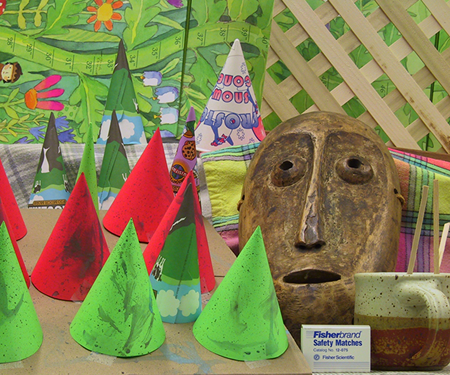
\includegraphics[width=0.9\linewidth]{Images/Chap_4/im2.png}
        \caption{Colored left image}
        \label{fig:color_cones_image}
    \end{subfigure}\hfill
    \begin{subfigure}[t]{0.5\linewidth}
        \centering
        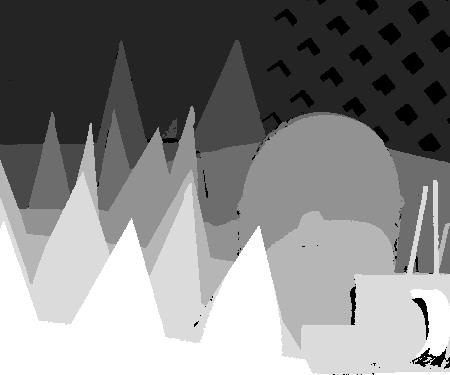
\includegraphics[width=0.9\linewidth]{Images/Chap_4/cluster.jpg}
        \caption{Proposed clustering of the image (\textit{k-means} with $K=8$)}
        \label{fig:cluster}
    \end{subfigure}
    \caption{Middlebury 2003 Cones left image, and a clustering computed from the disparity ground truth.}
    \label{fig:clustering_example}
\end{figure}

During our simulations, the segmentation contains $K=8$ different clusters. For every $k$ in $\opi1,K\cli$, $\rho_k$ is assigned an value between $0.9$ and $1$ in order to really emphasize on their correlation.\commanue{à mon avis tu peux regrouper cette phrase dans le milieu paragraphe précédent où tu décris ton modèle. Là elle se retrouve un peu isolée}

\begin{remark}
    The segmentation is based on the ground truth disparity map. This means that two objects with similar disparities located at opposite sides of the image will be considered as belonging to the same object and thus correlated. In practice, those pixels are never compared as we only measure the dissimilarity between small windows in a restricted disparity range. The clustering is thus only used at a \textit{local} scale. 
    
    Secondly, the segmentation allows to compute the Gaussian copula, which will be used to propagate the uncertainty models. We will validate the uncertainty propagation in \Cref{sec:montecarlo} with Monte Carlo samples using the same copula. As long as the copulas used are the same between the propagation and validation, it does not really matter which correlation matrix is used. We still tried to create a realistic but simple dependency model for the sake of the example, but it is not required from a theoretical point of view\commanue{là trop de remarques tue la remarques. Tu n'es pas obligé de faire des teasers sur tous les points que tu vas abordés. Je me limiterais à donner les infos qui correspondent au modèle de dépendence entre les images qui est le thème de la section. Si par la suite tu as besoin de réutiliser les copules, bah tu le dis.}.
\end{remark}

\section{Propagating the Uncertainty with Belief Functions and a Copula}
Having defined both marginal models for pixel intensities using possibility distributions as well as dependency models using copulas, we can now join them all to construct a multivariate uncertainty model, as seen in \Cref{sec:methods_for_joining_credal_sets}. We will see in this section how the multivariate models can then be used to compute the uncertainty regarding the cost curve. 

\subsection{From Multivariate Uncertainty Models to the Propagated Model}
We first detail how multivariate models are used to propagate uncertainty in the precise case. We will then do the same in the imprecise setting by analogy.

Consider a mapping $f:\X_1\times\X_2\rightarrow\mathcal{Z}$ from a product space $\X_1\times\X_2$ to a space $\mathcal{Z}$, which propagates multiple random variables $X_1$, $X_2$ to a new random variable $Z=f(X_1, ~X_2)$. In our case, $f$ will be the $\SAD$ cost function propagating the intensities to the matching cost. When considering precise probabilities, the probability of $Z$ on atoms $z$ is obtained by summing the probabilities of all events $X_1=x_1$, $X_2=x_2$ whose image by $f$ is $z$: 
\begin{align}\label{eq:precise_propagate_proba}
    \forall z\in\mathcal{Z}, P_Z(z)=\sum_{\substack{x_1,x_2\\z=f(x_1,x_2)}}P(x_1,x_2).
\end{align}
where $P(x_1,x_2)$ is the joint probability, which is linked to its marginals by a copula $C$. $P_Z$ is completely determined by evaluated every combination of atoms of $\X_1$ and $\X_2$.

\begin{example}\label{ex:propagated_probability}
    Consider the same setting as example \ref{ex:copulas}, where a dealer throws two coins in a separate room. The coins seem fair when looked at independently. In this example, a coin landing on heads rewards you with $1$€ (or any currency of your choice), and a coin landing on tails rewards you with $0$€. So you earn $2$€ if both coins land on heads, $1$€ if only one coin land on heads, and $0$€ if both coins land on tails. We are interesting in the uncertainty regarding you earnings, noted $Z$.
    
    In example \ref{ex:copulas}, we consider $3$ different cases, each leading to a different copula $C$ modelling the dependency between the probability $P_1$ of first coin and $P_2$ of the second coin. For each copula, we then computed the joint probability $P$.
    
    In the first case, where coin throws were independent, we saw that the joint probability $P$ was:\\
    \begin{minipage}[b]{0.5\linewidth}
    \begin{align*}
        & P(\text{heads}, ~\text{heads}) = 0.25\\
        & P(\text{heads}, ~\text{tails}) = 0.25
    \end{align*}
    \end{minipage}
    \begin{minipage}[b]{0.5\linewidth}
    \begin{align*}
        & P(\text{tails}, ~\text{tails}) = 0.25 \\
        & P(\text{tails}, ~\text{heads}) = 0.25
    \end{align*}
    \end{minipage}
    In that case, it holds that the probability $P_Z$ of our earnings are:
    \begin{align*}
        & P_Z(Z=2) = P(\text{heads}, ~\text{heads}) = 0.25\\
        & P_Z(Z=1) = P(\text{heads}, ~\text{tails}) + P(\text{tails}, ~\text{heads}) = 0.5 \\
        & P_Z(Z=0) = P(\text{tails}, ~\text{tails}) = 0.25
    \end{align*}
    
    In the second case, where coin throws were rigged to land on the same side, we saw that the joint probability $P$ was:\\
    \noindent
    \begin{minipage}[b]{0.5\linewidth}
    \begin{align*}
        & P(\text{heads}, ~\text{heads}) = 0.5\\
        & P(\text{heads}, ~\text{tails}) = 0
    \end{align*}
    \end{minipage}
    \begin{minipage}[b]{0.5\linewidth}
    \begin{align*}
        & P(\text{tails}, ~\text{tails}) = 0.5\\
        & P(\text{tails}, ~\text{heads}) = 0 
    \end{align*}
    \end{minipage}
    Following the same methodology, we have:\\
    \noindent\begin{minipage}[b]{0.33\linewidth}
    \begin{align*}
        & P_Z(Z=2) = 0.5
    \end{align*}
    \end{minipage}
    \begin{minipage}[b]{0.33\linewidth}
    \begin{align*}
        & P_Z(Z=1) = 0
    \end{align*}
    \end{minipage}
    \begin{minipage}[b]{0.33\linewidth}
    \begin{align*}
        & P_Z(Z=0) = 0.5
    \end{align*}
    \end{minipage}
    
    In the third case, where coin throws were rigged to land on opposite sides, we saw that the joint probability $P$ was:\\
    \noindent\begin{minipage}[b]{0.5\linewidth}
    \begin{align*}
        & P(\text{heads}, ~\text{heads}) = 0\\
        & P(\text{heads}, ~\text{tails}) = 0.5
    \end{align*}
    \end{minipage}
    \begin{minipage}[b]{0.5\linewidth}
    \begin{align*}
        & P(\text{tails}, ~\text{tails}) = 0\\
        & P(\text{tails}, ~\text{heads}) = 0.5
    \end{align*}
    \end{minipage}
    Therefore:\\
    \begin{minipage}[b]{0.33\linewidth}
    \begin{align*}
        & P_Z(Z=2) = 0
    \end{align*}
    \end{minipage}
    \begin{minipage}[b]{0.33\linewidth}
    \begin{align*}
        & P_Z(Z=1) = 1
    \end{align*}
    \end{minipage}
    \begin{minipage}[b]{0.33\linewidth}
    \begin{align*}
        & P_Z(Z=0) = 0
    \end{align*}
    \end{minipage}
\end{example}

Determining every $(x_1, x_2)$, whose image by $f$ equals $z$, is not always trivial. This becomes even more complex when considering $n>2$ marginal variables. Similarly, the joint probability $P(x_1,x_2)$ is computed using a H-volume, which is the sum of $2^n$ terms, thus also increasing exponentially with the dimension.

There are multiple ways of extending \cref{eq:precise_propagate_proba} to the imprecise setting, as there are multiple ways of aggregating imprecise models using a copula. We presented\commanue{tu emploies bcp cette formule, donc de temps en temps described/} in \Cref{chap:joining_credal_sets} three methods for joining marginal credal sets, creating three different multivariate credal sets $\M_{robust}$, $\M_{mass}$ and $\M_{agg}$.

The robust approach of extending \cref{eq:precise_propagate_proba} is based on the robust approach from \Cref{sec:robust_method}. Given $n$ marginal credal sets $\M_i$, we can join them using a copula $C$ into a credal set $\M_{robust}$ as in \eqref{eq:robust_set}. The propagated uncertain model $\M^Z_{robust}$ is then defined as:
\begin{align}
    \M^Z_{robust} = \{P_Z~|~\forall z\in Z, ~P_Z(z)=\sum_{\substack{x_1 \enum x_n\\z=f(x_1 \enum x_n)}}P(x_1 \enum x_n), ~P\in\M_{robust}\}
\end{align}
Practically, this set is computed by sampling every probability $P_i$ from each marginal credal set $\M_i$ and joining them using \hyperref[theorem:sklar]{Sklar's Theorem} into a multivariate probability $P$. Then for each $z=P(x_1 \enum x_n)$, we can compute $P_Z$ from $P$ using \eqref{eq:precise_propagate_proba}. In short, each sample $(P_1 \enum P_n)$ leads to a new $P$, itself leading to a new $P_Z$. Sampling through every $(P_1 \enum P_n)$ thus leads to the estimation of the uncertain model of $Z$. This method is complicated to compute, but correctly propagates the uncertainty.

We saw that it was easier to compute $\M_{mass}$ than $\M_{robust}$. Another way\commanue{mot de liaison entre les deux phrase. So another way or Thus another way} of approximating the uncertainty model of $Z$ is to compute it using $\M_{mass}$. This is done by replacing the probability on atoms from \cref{eq:precise_propagate_proba} with the joint mass $m_\times$ from \cref{eq:joint_mass} \cite{gray_dependent_2021}. Consider $n$ uncertain variables $X_i$, each modeled by a mass distribution function whose $j$-th focal set is noted $a^i_j$. Given their multivariate mass $m_\times$, it is possible to compute the mass distribution function $m_Z$ of a random set $Z=f(X_1 \enum X_n)$ as:
\begin{align}
    \forall a^Z\subseteq\mathcal{Z}, m_Z(a^Z) = \sum_{\substack{a^1_i \enum a^n_j\\a^Z=f(a^1_i \enum  a^n_j)}}m_\times(a^1_i \enum a^n_j)\label{eq:mass_propagated}
\end{align}
leading to a credal set $\M_{mass}^Z$:
\begin{align}
    \M_{mass}^Z &= \{~P_Z~|~\forall A\subseteq\mathcal{Z},~P_Z(A)\geqslant \sum_{a^Z\subseteq A}m_Z(a^Z)\}\\
    &=\{~P_Z~|~\forall A\subseteq\mathcal{Z},~P_Z(A)\geqslant \sum_{\substack{a^1\enum a^n \\ f(a_1\enum a_n)\subseteq A}}m_\times(a^1\enum a^n)~\}
\end{align}

In order to compute the propagated mass $m_Z$ (and its associated belief function) from \cref{eq:mass_propagated}, two difficulties arise. The first one is to determine what the focal sets $a_Z$ of $m_Z$ will be, which corresponds to the subscript $a^Z=f(a^n_1 \enum  a^n_j)$ of the previous sum. Computing the image of $f$ for every combination of focal sets $(a^1_i \enum a^n_j)$ is even more difficult than in the precise case, as we are computing images of sets instead of real numbers. The second difficulty is to compute the joint mass $m_\times$, as in the case of the $\SAD$ it requires to compute the H-volume of an $18$-copula. Those difficulties will be addressed in the following sections \ref{sec:propagated_focal_sets} and \ref{sec:propagated_masses}

We saw in \Cref{chap:joining_credal_sets} that in the situation where marginals are possibility distributions, $\M_{mass}$ and $\M_{agg}$ have the same bounds on Cartesian products of events (see \cref{eq:inclusion_necessity}). We will thus only compute the lower bounds $Bel_\times$ of $\M_{mass}$ as it directly provides the bounds of $\M_{agg}$ on those events\commanue{tu n'as pas inversé $\M_{mass}$  et $\M_{agg}$ dans ta phrase ? $\M_{agg}$ c'ets pas celui qui est plus facile à calculer}.

\subsection{Determining the Propagated Focal Sets}\label{sec:propagated_focal_sets}
In this section, we will detail how we compute the $\SAD$ image of marginal focal sets. Computing the image of sets needs to be treated with caution in the general case. However in our case, because we chose marginal focal sets with a simple expression, and because we are using a relatively regular cost function, computing the image is significantly easier.

Given a pixel $p$, we consider the mass distribution $m_p$ of \cref{eq:pixel_mass} and its two focal sets $a_1^p$ and $a_2^p$ from \cref{eq:pixel_mass}. For every pair of pixels $p\in I_L, q\in I_R$, we note $\AD_{pq}=|i_p - i_q|$, where $i$ refers to a pixel's intensity. Given $m_p$, There exist $3$ focal sets related to the absolute difference:
\begin{itemize}
    \item $a^{\AD}_1$ is the image of the AD of $a^p_1$ and $a^q_1$
    \item $a^{\AD}_2$ is the image of the AD of $a^p_2$ and $a^q_1$ or $a^p_1$ and $a^q_2$
    \item  $a^{\AD}_3$ is the image of the AD of $a^p_2$ and $a^q_2$
\end{itemize}
The non-monotonicity of the absolute value around $0$ needs to be taken into account to compute their exact image through the AD. Indeed, if a value $x$ is in $[-1,1]$, then its absolute value will be in $[0,1]$. Applying this remark to the AD yields the following focal sets:
\begin{align*}
    a^{\AD}_1&=\opi\AD_{pq},~\AD_{pq}\cli\,,\\
    a^{\AD}_2&=\opi\max(0, \AD_{pq} - 1),~\AD_{pq} + 1\cli\,,\\
    a^{\AD}_3&=\opi\max(0, \AD_{pq} - 2),~\AD_{pq} + 2\cli\,,
\end{align*}

Focal sets of the final $\SAD$ are then computed by simply summing the bounds of the $9$ AD focal sets (as in \Cref{fig:SAD}), for every combination $(a^{\AD_1}_{k_1}\enum a^{\AD_9}_{k_9})$ of those focal sets:
\begin{align}
    a^\SAD=\sum_{i=1}^9a^{\AD_i}_{k_i}
\end{align}

\begin{remark}
    In many cases, different combinations of $\AD$ focal sets will lead to the same $\SAD$ focal set. Actually, if every $\AD$ is greater than $2$\commanue{alors je ne suis pas sure de comprendre} (so that each $a^\AD_i$ is symmetric with regards to its $\AD$) there will only be $19$ focal sets $a^\SAD$ for the $\SAD$, and they are of the following form:
    \begin{align}\label{eq:nested_SAD}
        a^\SAD = \opi\SAD-t,\SAD+t\cli,\text{ with }t\in\opi0, ~18\cli
    \end{align}
    In comparison, there are $3^9=19683$ different combinations of $\AD$ focal sets.
\end{remark}

\begin{remark}\commanue{pourquoi tu mets ce qui concerne SAD dans des remarques ?}
    In the previous remark, we established that when every $\AD$ is greater than $2$, it holds that:
    \begin{align*}
        a^\SAD = \opi\SAD-t,\SAD+t\cli,\text{ with }t\in\opi0, ~18\cli
    \end{align*}
    This equation translates the fact that focal sets of the $\SAD$ form an increasing family of events. This also means that $\Bel_\SAD$ is actually a necessity function. We can thus compute a possibility distribution $\pi_\SAD$ to represent the uncertainty of the $\SAD$. This can be useful for graphically representing the uncertainty of the $\SAD$, if we later need to build joint uncertainty models using the $\SAD$, or if we want to propagate the $\SAD$ uncertainty even further.
    
    We proved in \cite{malinowski_uncertainty_2024} that in order to propagate marginal possibility distributions $\pi_i$ into a possibility distribution $\pi_Z$ using a copula and a propagating function $f$, a sufficient condition was that\commanue{tu n'as pas deux conditions dans ce qui suit}:
    \begin{itemize}
        \item $f$ is a monotone function applied to a linear combination $\alpha_1X_1+\dots+\alpha_nX_n+\beta$ of marginal variables $X_i$
        \item Each $\pi_i$ is symmetrical and uni-modal (meaning that all values $x_i$ such that $\pi_i(x_i)=1$ are adjacent). For instance all triangular possibility distributions verify this condition
    \end{itemize}
    Here is an example of an uni-modal symmetrical possibility
    \centering{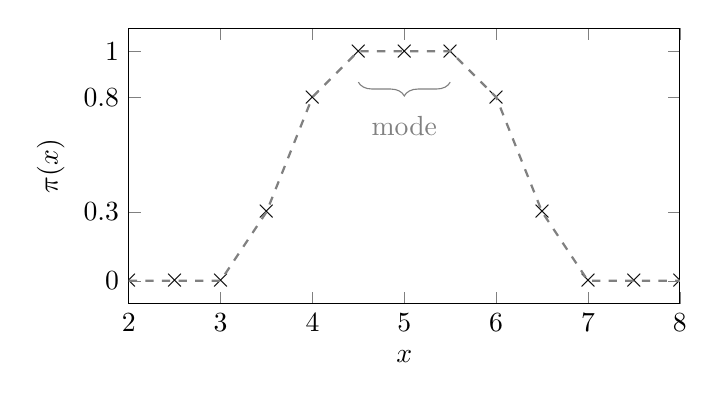
\begin{tikzpicture}[scale=1]
        \begin{axis}[%
          xlabel=$x$,
          ylabel=$\pi(x)$,
          xmin=2, xmax=8,
          ymin=-0.05, ymax=0.55,
          ytick={0, 0.15, 0.4, 0.5},
          yticklabels={$0$, $0.3$, $0.8$, $1$},
          scale only axis,
          width=7cm, height=3.5cm,
          ],
          \node (a) at (2, 0) {$\times$};
          \node (b) at (2.5, 0) {$\times$};
          \node (c) at (3, 0) {$\times$};
          \node (d) at (3.5, 0.15) {$\times$};
          \node (e) at (4, 0.4) {$\times$};
          \node (f) at (4.5, 0.5) {$\times$};
          \node (g) at (5, 0.5) {$\times$};
          \node (h) at (5.5, 0.5) {$\times$};
          \node (i) at (6, 0.4) {$\times$};
          \node (j) at (6.5, 0.15) {$\times$};
          \node (k) at (7, 0) {$\times$};
          \node (l) at (7.5, 0) {$\times$};
          \node (m) at (8, 0) {$\times$};
          
          \draw [thick, dashed, gray] (a.center) -- (b.center) -- (c.center) -- (d.center) -- (e.center) -- (f.center) -- (g.center) -- (h.center) -- (i.center) -- (j.center) -- (k.center) -- (l.center) -- (m.center) ;
          \draw [decorate,decoration={brace,amplitude=5pt,mirror,raise=1ex},gray] (f.south) -- (h.south) node[midway,yshift=-2em]{\color{gray}{mode}};
        \end{axis}
    \end{tikzpicture}}
\end{remark}

\subsection{Computing the Mass of Propagated Focal Sets}\label{sec:propagated_masses}
%\section{Leveraging Specificities to Accelerate Computations}
Now that the bounds of the $\SAD$ have been computed\commanue{alors moi j'ai compris qu'on avait calculé les focal sets. J'ai pas bien vu le calcul des bornes}, we need to compute the associated mass. Computing the joint mass over two $3 \times 3$ windows is significantly more complex. For each combination of marginal focal sets, the joint mass $m_{\times}$ is computed using the H-volume of an $18$-copula, involving a sum of $2^{18}$ terms. Given that the uncertainty of each of the 18 pixels is represented by $2$ focal sets, we need to evaluate $2^{18}$ combinations of these focal sets in total\commanue{c'est juste moi qui comprends pas la subtilité }. This computation can thus become quite costly in memory and computation time, especially when computing it over a whole image.

In the case of the family of Gaussian copulas, their expression given by \cref{eq:gaussian_copula} show that we need to compute the multivariate CDF. An $18$-variate Gaussian CDF does not possess a known analytic formula, it is thus computed by integrating its density (so integrating a $18$-variate function), as expressed below:
\begin{align}\label{eq:gaussian_cdf}
    F(x_1 &\enum x_{18}) =\nonumber\\ &\int_{-\infty}^{x_1}\dots\int_{-\infty}^{x_{18}}\frac{1}{\sqrt{(2\pi)^{18}|R|}}\exp(-\frac{1}{2}\begin{bmatrix}x_1 & \dots & x_{18}\end{bmatrix}R^{-1}\begin{bmatrix}x_1 \\ \dots \\ x_{18}\end{bmatrix})dx_1\dots dx_{18}
\end{align}
Where $|R|$ is the determinant of $R$. Computing this CDF can quickly become time-consuming ($40ms$ on average\footnote{With an AMD EPYC7713  64-Core Processor at 2GHz, using Python and the SciPy library}). For each pixel and each disparity, we saw that we need to compute the joint mass of $2^{18}$ focal sets, each time necessitating $2^{18}$ evaluation of its copula. Because there are around $170\,000$ pixels and $60$ disparities to be evaluated, the processing time is too large to be computed as such. We will instead see that we can leverage specificities of our problem to drastically reduce the computation time.
 
The first idea is to notice than if we can divide our variables into multiple mutually independent sets of variables, then the evaluation of the $18$-copula can be separated into the evaluation of multiple lower dimension copulas. To verify this statement consider the following independent sets of variables $\{X_1 \enum X_k\}$ and $\{X_{k+1} \enum X_n\}$ with $k\in\opi1,n-1\cli$. Let $F_1 \enum  F_n$ be their marginals CDF. And let $F_{(1 \enum n)}$ be the joint CDF of all variables, $F_{(1 \enum k)}$ the joint CDF of the first set of variables and $F_{(k+1 \enum n)}$ the joint CDF of the second set. The two sets are independent means that for all $(x_1 \enum x_n)\in\X_1\tdt\X_n$ it holds that:
\begin{align*}
    F_{(1 \enum n)}(x_1 \enum x_n) = F_{(1 \enum k)}(x_1 \enum x_k)\cdot F_{k+1 \enum n}(x_{k+1} \enum x_n)
\end{align*}
Using Sklar's theorem, there exist a $n$-copula $C$, a $k$-copula $C'$ and a $n-k$-copula $C''$ respectively linking $F_{(1 \enum n)}$, $F_{(1 \enum k)}$, and $F_{(k+1 \enum n)}$ to their marginals:
\begin{align}
    C(F_1(x_1) \enum F_n(x_n)) = C'(F_1(x_1) \enum F_k(x_k))\cdot C''(F_{k+1}(x_{k+1}) \enum F_n(x_n))\label{eq:copula_factorizing}
\end{align}

\begin{remark}
    We stated earlier that we did not considered vine copulas \cite{czado_vine_2022}, which are a way of constructing multivariate copulas by composition of bivariate (conditional) copulas. The decomposition $C$ into $C'$ and $C''$ actually follows the same idea of decomposing a copula into smaller ones. So even though we are not using vine copulas, we use a similar philosophy in our computations.
\end{remark}

Establishing \cref{eq:copula_factorizing} becomes interesting once we put it in relation with the following property:
\begin{proposition}[H-Volume factorizing]\label{prop:hvol_factorizing}
    Let $1<k<n$. If a $n$-copula $C$ can be expressed as the product of a $k$-copula $C'$ and a $(n-k)$-copula $C''$, then the H-volume of $C$ is the product of the H-volume $H'$ of $C'$ and the H-volume $H''$ of $C''$. This means that for all $(u_1 \enum u_n)\in[0,1]^n$ and for all $(v_1 \enum v_n)\in[0,1]^n$ such that $u_i\leqslant v_i$, it holds that:
    \begin{align}
        H_{u_1 \enum u_n}^{v_1 \enum v_n} = {H'}_{u_1 \enum u_k}^{v_1 \enum v_k}\cdot{H''}_{u_{k+1} \enum u_n}^{v_{k+1} \enum v_n}
    \end{align}
\end{proposition}
\begin{proof}
    Let $1<k<n$, $C$ a $n$-copula, $C'$ a $k$-copula and $C''$ a $n-k$ copula. $H$, $H'$, $H''$ are the respective H-volume of $C$, $C'$, $C''$. then
    \begin{align*}
        %{H'}_{u_1 \enum  u_k}^{v_1 \enum  v_k}\times {H''}&_{u_{k+1} \enum  u_n}^{v_{k+1} \enum  v_n} = \left(\sum_{w_i\in\Pi_{i=1}^{k}\{u_i,v_i\}}(-1)^{|\{w_i~|~w_i=u_i\}|}C'(w_1 \enum w_k)\right)\\
        {H'}
        \begin{matrix}
            v_1 \enum  v_k\\
            u_1 \enum  u_k
        \end{matrix}
        \cdot {H''}&
        \begin{matrix}
            v_{k+1} \enum  v_n\\
            u_{k+1} \enum  u_n
        \end{matrix}= \left(\sum_{w_i\in\Pi_{i=1}^{k}\{u_i,v_i\}}(-1)^{|\{w_i~|~w_i=u_i\}|}C'(w_1 \enum w_k)\right)\\
        &\times\left(\sum_{w_j\in\Pi_{j=k+1}^{n}\{u_j,v_j\}}(-1)^{|\{w_j~|~w_j=u_j\}|}C''(w_{k+1} \enum w_n)\right)\\
        =& \sum_{w_i\in\Pi_{i=1}^{k}\{u_i,v_i\}}\times\sum_{w_j\in\Pi_{j=k+1}^{n}\{u_j,v_j\}}(-1)^{|\{w_i~|~w_i=u_i,~i\leqslant k\}|}\\
        &\times(-1)^{|\{w_j~|~w_j=u_j,~ j>k\}|}C'(w_1 \enum w_k)C''(w_{k+1} \enum w_n)\\
        =&\sum_{w_i\in\Pi_{i=1}^{n}\{u_i,v_i\}}(-1)^{|\{w_i~|~w_i=u_i\}|}C'(w_1 \enum w_k)\\
        &\times C''(w_{k+1} \enum w_n)\\
        =&H
        \begin{matrix}
            v_1 \enum  v_n\\
            u_1 \enum  u_n
        \end{matrix}
        %=&H_{u_1 \enum  u_n}^{v_1 \enum  v_n}
    \end{align*}
\end{proof}
Using the result of proposition \ref{prop:hvol_factorizing}, we can now compute the joint mass as a product of two lower dimension copulas. It is easier to compute as we only integrate a $k$-dimensional function and a $n-k$-dimensional function, instead of a $n$-dimensional one. Similarly the $H$ volume is not the sum of $2^{18}$ terms anymore, but the sum of $2^{k}$ and $2^{n-k}$ terms.

For comparison, consider that we can split the aforementioned Gaussian $18$-copula into two Gaussian $9$-copula. Computing the value of single mass used to take around $10\,500s$, but now takes around $6s$, so around $1\,700$ times faster. This demonstrates the substantial time savings achieved by decomposing the problem into smaller, independent parts. This improvements apply directly to our application. Indeed \cref{eq:correlation} yields the following correlation between two pixels $p$, $q$ given the segmentation $S$:
\begin{equation*}
    \sigma(p, q) =
    \begin{cases}
        1 &\text{ if }p=q,\\
        \rho_k, &\text{ if } p\ne q\text{ and }S(p)=S(q)\,, \\
        0 & \text{otherwise}\,.
    \end{cases}
\end{equation*}
From this, we can split the set $\{p_1 \enum p_{18}\}$ of pixels in at most $K=8$ mutually independent sets $S_k = \{p_i~|~S(p_i)=k\}$, each set containing pixels from the same cluster. We can thus compute the H-volume of each cluster independently.

Another additional way of reducing the computation time is to avoid computing the same $H$-volume multiple times. Consider a set $S_k$ with $k_L$ pixels from the left image and $k_R$ pixels from the right image. The correlation matrix $R_k$ for this cluster is:
\begin{equation}
    R_k=\begin{pmatrix}
        1 &  & \rho_k & \dots & \rho_k\\
         & & & & \vdots\\
        \rho_k &  & 1 & & \rho_k\\
        \vdots &  &  & & \\
        \rho_k & \dots & \rho_k &  & 1
    \end{pmatrix}\label{eq:corr_matrix_sym}
\end{equation}
which implies that the Gaussian $(k_L+k_R)$-copula for this set is symmetrical. The joint mass $m^{S_k}_\times$ of this set is then also symmetrical. Pixels from the left image will share the same mass $m_L$ for their two focal sets and pixel from the right image will also share the same mass $m_R$, therefore computing $m^{S_k}_\times$ on every possible combination of cumulative masses is redundant. 
\begin{example}
    Let us imagine a set $S_k$ with $k_L=2$ pixels $p_1$, $p_2$ from the left image and $k_R=2$ pixels $p_3$, $p_4$ from the right image. Each pixel $p_i$ has two focal sets $a^i_1$ and $a^i_2$.
    We know that:
    \begin{align*}
        m_L(a_1^1) &= m_L(a_1^2) \qquad m_L(a_2^1) = m_L(a_2^2)\\
        m_R(a_1^3) &= m_R(a_1^4) \qquad m_R(a_2^3) = m_R(a_2^4)
    \end{align*}
    Because of the symmetry of the Gaussian $4$-copula of the set $S_k$, the joint mass $m^{S_k}_\times$ computed as the H-volume on cumulative masses (\cref{eq:joint_mass}) verifies:
    \begin{align*}
        m^{S_k}_\times(a_1^1, a_2^2, a_1^3, a_2^4) &= H
        \begin{matrix}
            m_L(a_1^1), & m_L(a_1^1)+m_L(a_2^2), & m_R(a_1^3), & m_R(a_1^4)+m_R(a_2^4)\\
            0, & m_L(a^2_1), & 0, & m_R(a_1^4)
        \end{matrix}\\
        &=H
        \begin{matrix}
            m_L(a_1^1)+m_L(a_2^1), & m_L(a_1^2), & m_R(a_1^3)+m_R(a_2^3), & m_R(a_1^4)\\
            m_L(a^1_1), & 0, & m_R(a_1^3), & 0
        \end{matrix}\\
        &\text{(by symmetry of the copula)}\\
        &= m^{S_k}_\times(a_2^1, a_1^2, a_2^3, a_1^4)
    \end{align*}
    We can see that we do not need to compute $m^{S_k}_\times$ on every possible combination of focal sets as many combination have the same joint mass $m^{S_k}_\times$.
\end{example}
For each set $S_k$, we only have to compute $(k_L+1)(k_R+1)$ values of $m^{S_k}_\times$ rather than $2^{k_L+k_R}$.

We saw that it was complex to compute the joint mass of the $\SAD$. However, by taking advantage of the potential factorization of the copula into smaller copulas, and by leveraging some symmetries of the problem, we can greatly reduce the time and number of computations required.

\section{Results and discussions}
In the previous section, we presented how we can use $\M_{robust}$ and $\M_{mass}$ to propagate the uncertainty from the input images into the uncertainty of the $\SAD$. Evaluating this uncertainty for every pixel and every considered disparity results in the uncertainty models of every value of the cost volume (see \cref{eq:cost_volume} from \Cref{sec:stereo_matching} for more details on the cost volume). We saw in \Cref{sec:necessity_functions} that $\M_{mass}$ and $\M_{robust}$ are different credal sets, and that neither set is guaranteed to be included in the other. This section will then compare the different models and see if $\M^Z_{mass}$ can be used to approximate $\M^Z_{robust}$. \Cref{sec:envelopes_plausibility} will present visualisations of  $\M^Z_{mass}$ using plausibility envelopes. \Cref{sec:montecarlo} will present visualisations of $\M^Z_{robust}$ using Monte Carlo samples and compare them to the plausibility envelopes. Finally, \Cref{sec:sad_improvements} will estimate the potential improvements unlocked by estimating the uncertainty.

\subsection{Envelopes Defined by Plausibility Levels}\label{sec:envelopes_plausibility}
Having defined efficient ways of computing the $\SAD$ focal sets in \Cref{sec:propagated_masses} and the joint mass in \ref{sec:propagated_focal_sets}, we can determine the belief function $\Bel_\SAD$ associated to every estimation of the $\SAD$ between two $3\times3$ windows. $\Bel_\SAD$ is deducted from the mass $m^\SAD_\times$ computed in \cref{eq:mass_propagated}.

For each pixel $p_L=(row, ~col)$ in the left image and for each disparity $d$, we calculated the $\SAD$ cost between the window centered on $p_L$ in the left image and the window centered on $p_R=(row, ~col+d)$ in the right image. We are usually interested in going through each considered disparity $d$ to obtain the cost curve for pixel $p_L$. From this cost curve, a \textit{winner-takes-all} strategy is applied to find the correct disparity. Due to its interest, we want to visualise the uncertainty of the entirety of the cost curve, not just a single value.

It can be hard to graphically represent focal sets, or similarly belief functions, especially when there is a large number of sets to consider. We are usually more keen to represent uncertainty on singletons, as we do with probability densities, possibility distributions or, to a certain extent, p-boxes (although in that case singletons represent cumulative events). Following that logic, we will consider the plausibility of singletons as a way of representing the uncertainty graphically.
\begin{remark}
    Considering the belief on singletons instead of the plausibility does not make much sense as the belief of singletons is null. The only exception is the precise $\SAD$ value, because it is the only singleton that is also a focal set.
\end{remark}
We will first explain how we  graphically represent the uncertainty on the special case of possibility distributions, and then extend this representation to all $\SAD$ belief functions. 

As shown in \Cref{sec:propagated_focal_sets}, focal sets representing the $\SAD$ uncertainty are defined as intervals containing the ``precise'' $\SAD$ value. We saw in a remark from \Cref{sec:propagated_focal_sets} that the uncertainty of the $\SAD$ could be represented by a possibility distribution $\pi_\SAD$ in the special case where all $\AD$ leading to the $\SAD$ are greater that $2$. In this case, we can easily plot this possibility distribution, at least for a few degrees of possibility. Given a degree of possibility $\gamma$, we plot the bounds of the largest interval $I_\gamma=[\underline{I}_\gamma, \overline{I}_\gamma]$ whose possibility is greater than $\gamma$. The possibility measure is computed as $\Pi_\SAD(A)=\sup_{z\in A}\pi_\SAD(z)$ or $\Pi_\SAD(A)=\sum_{a\cap A\neq\emptyset}m^\SAD_\times(a)$ using \cref{eq:bel_pl}. This way, given $\gamma\in[0,1]$, the bounds $\underline{I}_\gamma, \overline{I}_\gamma$ to plot are:
\begin{align}\label{eq:possibility_bounds}
    \underline{I}_\gamma = \argmin_{z}\{\pi_\SAD(z)\geqslant\gamma\}, \qquad \overline{I}_\gamma = \argmax_{z}\{\pi_\SAD(z)\geqslant\gamma\}
\end{align}
Because focal sets of $\pi_\SAD$ are increasing intervals, then every $\SAD$ value between $\underline{I}_\gamma$ and $\overline{I}_\gamma$ will have a possibility superior to $\gamma$. The bounds thus define the envelope of values with a degree of possibility greater than $\gamma$. Plotting envelopes for different values of $\gamma$ allows to visualize a representation of the $\SAD$ uncertainty. We will define the envelopes in the following, but readers can already have a broad idea of what those envelopes look like by looking at \Cref{fig:belief_curves}. 

In \cref{eq:possibility_bounds}, $\underline{I}_\gamma$ and $\overline{I}_\gamma$ are the upper and lower bounds of the same focal set. If we relax this constraint, then we can extend this definition of $\underline{I}_\gamma, \overline{I}_\gamma$ to any type of $\SAD$ plausibility (or equivalently belief) function $\Pl_\SAD$. For all focal sets $a=[\underline{a}, \overline{a}]$ of the $\SAD$ plausibility function, the bounds $\underline{I}_\gamma, \overline{I}_\gamma$ are defined as:
\begin{align}\label{eq:belief_bounds}
    \underline{I}_\gamma = \min\{\underline{a} ~|~ \Pl_\SAD([\underline{a}, \overline{a}])\geqslant\gamma\}, \qquad \overline{I}_\gamma = \max\{\overline{a} ~|~ \Pl_\SAD([\underline{a}, \overline{a}])\geqslant\gamma\}
\end{align}

\begin{remark}
    \Cref{eq:belief_bounds} details how we chose to represent a plausibility function (or equivalently a credal set) by some envelopes. One can wonder if we can reconstruct the plausibility function from the envelopes. It is straightforward to see that it is the case if and only if the plausibility function is a possibility measure, because it is then fully determined by its values on singletons.
    
    However if the plausibility is not a possibility measure, then the possibility distribution $\pi'$ defined by envelopes induces the smallest credal set $\M(\pi')$ containing $\M(\Pl_\SAD)$. In that regard, we chose to represent a plausibility by its best outer approximating possibility.
\end{remark}
Now that the we decided on how to plot our uncertainty models, we can present some results. We arbitrarily considered different values for plausibility levels $\gamma$:
\begin{itemize}
    \item The first value is $\gamma=1$. It corresponds to the $\SAD$ value with the highest degree of possibility. This value is unique in our case, and corresponds to the $\SAD$ value that would have been computed without considering the uncertainty.
    \item We then consider values $\gamma=0.9$ and $\gamma=0.85$. They allow to give an estimation of the dispersion of envelopes with high plausibility. With them, we can estimate if highly plausible values are near the $\SAD$ values or not.
    \item $\gamma=0.5$ gives a moderate plausibility estimation. From a credal set point of view, the probability that the $\SAD$ value lies in this set is at least $0.5$.
    \item The last value is $\gamma=0$. For this value, the inequalities in \cref{eq:belief_bounds} are actually strict (otherwise the inequality is verified by all imaginable values). These bounds represent the support of the plausibility function, or in other words, the range of values covered by focal sets.
\end{itemize}

\begin{figure}
    \centering
    \begin{subfigure}[t]{0.48\linewidth}
        \centering
        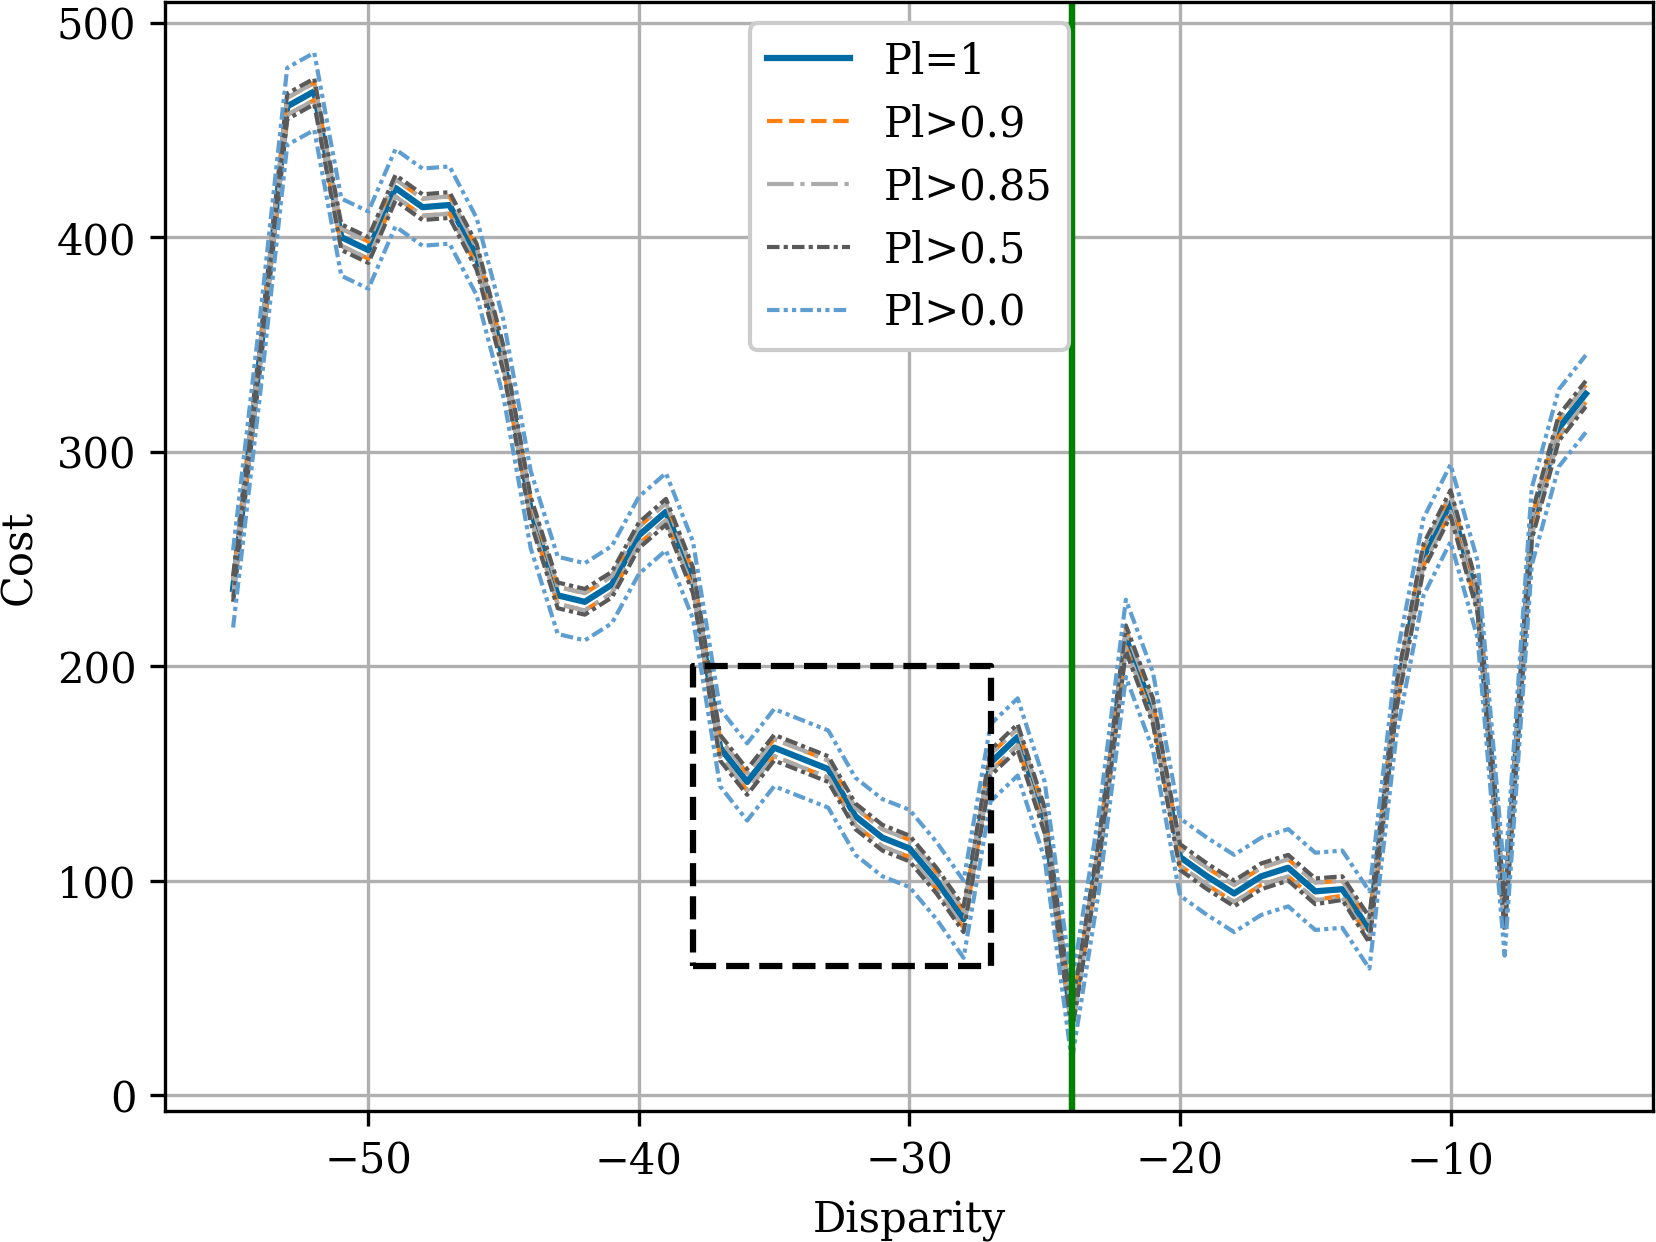
\includegraphics[width=\linewidth]{Images/Chap_4/bel_independence_100_120.png}
        \caption{$\SAD$ envelopes using the product Copula}
        \label{fig:belief_independence}
    \end{subfigure}\hfill
    \begin{subfigure}[t]{0.48\linewidth}
        \centering
        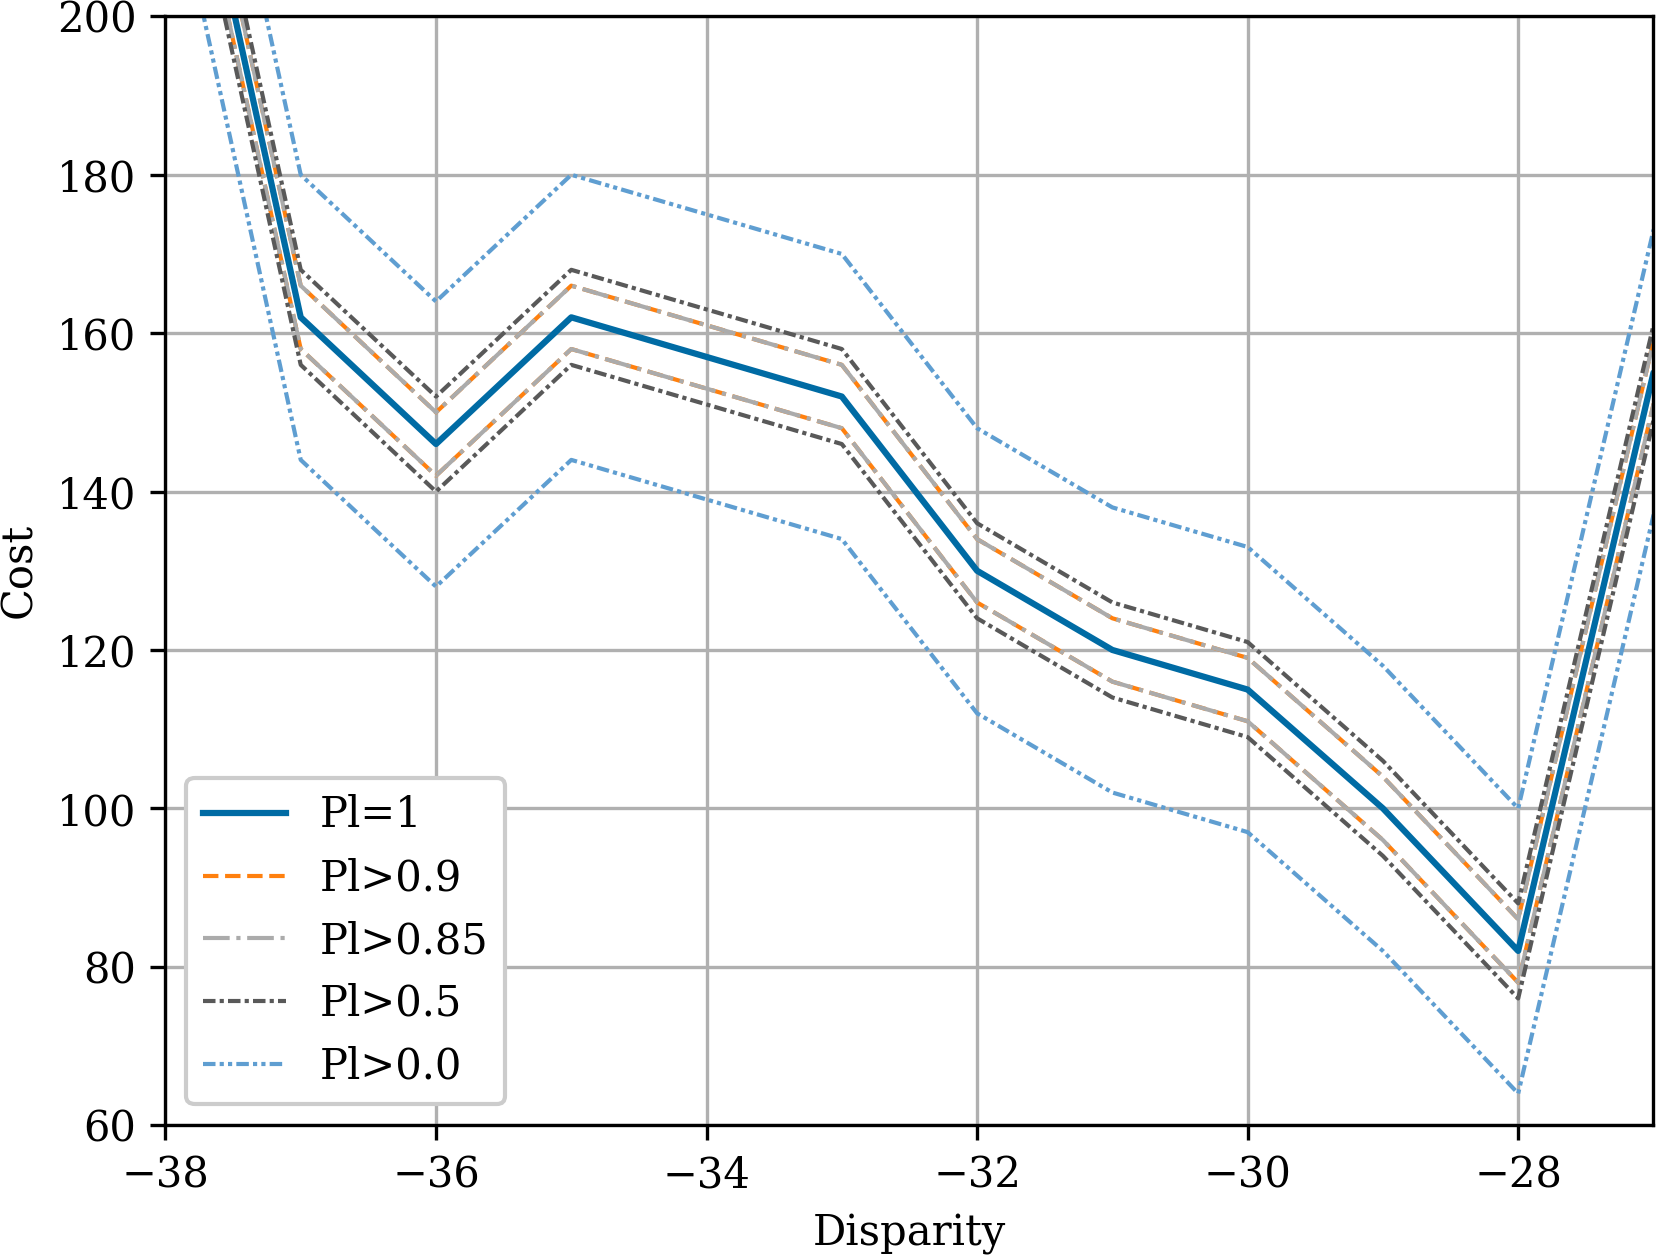
\includegraphics[width=\linewidth]{Images/Chap_4/bel_independence_100_120_zoom.png}
        \caption{Detailed view of the rectangular section of \ref{fig:belief_independence}}
        \label{fig:belief_independence_zoom}
    \end{subfigure}
    \begin{subfigure}[t]{0.48\linewidth}
        \centering
        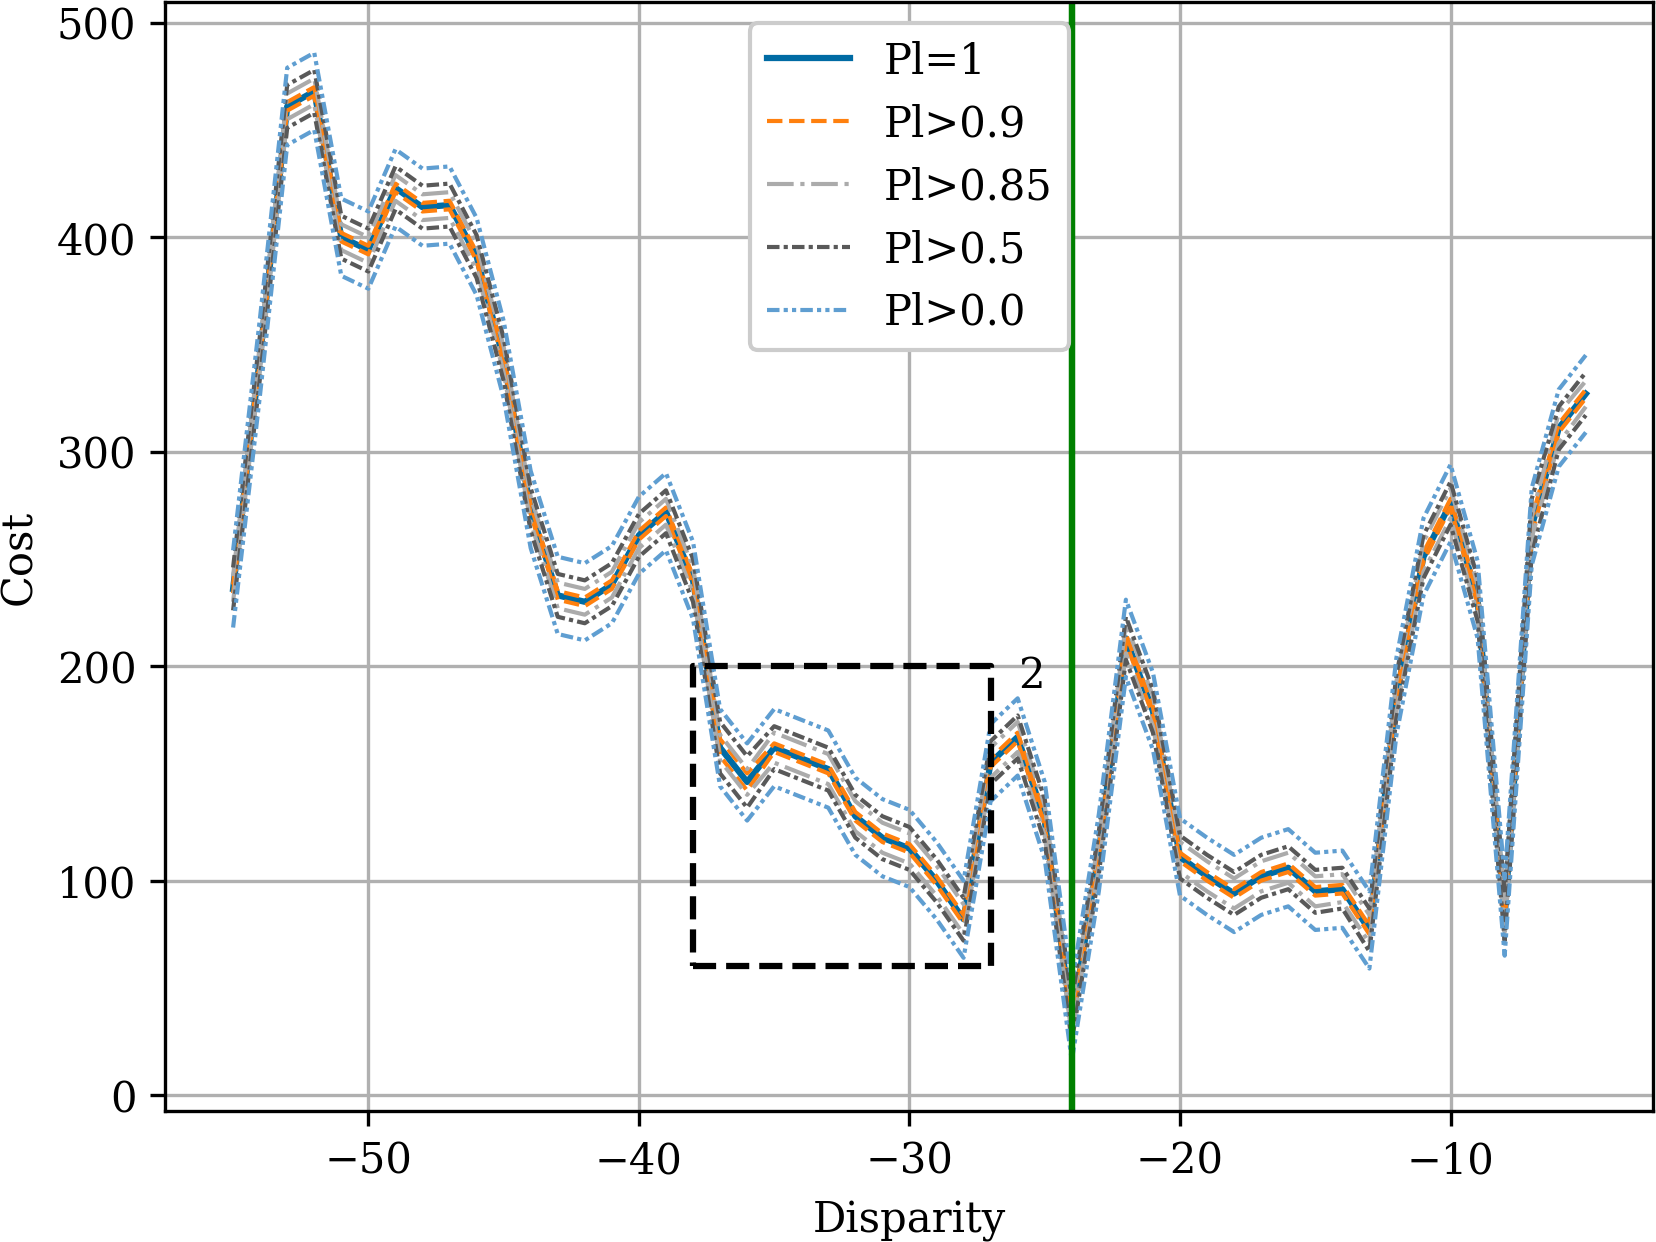
\includegraphics[width=\linewidth]{Images/Chap_4/bel_100_120.png}
        \caption{$\SAD$ envelopes using the Gaussian Copula}
        \label{fig:belief_gaussian}
    \end{subfigure}\hfill
    \begin{subfigure}[t]{0.48\linewidth}
        \centering
        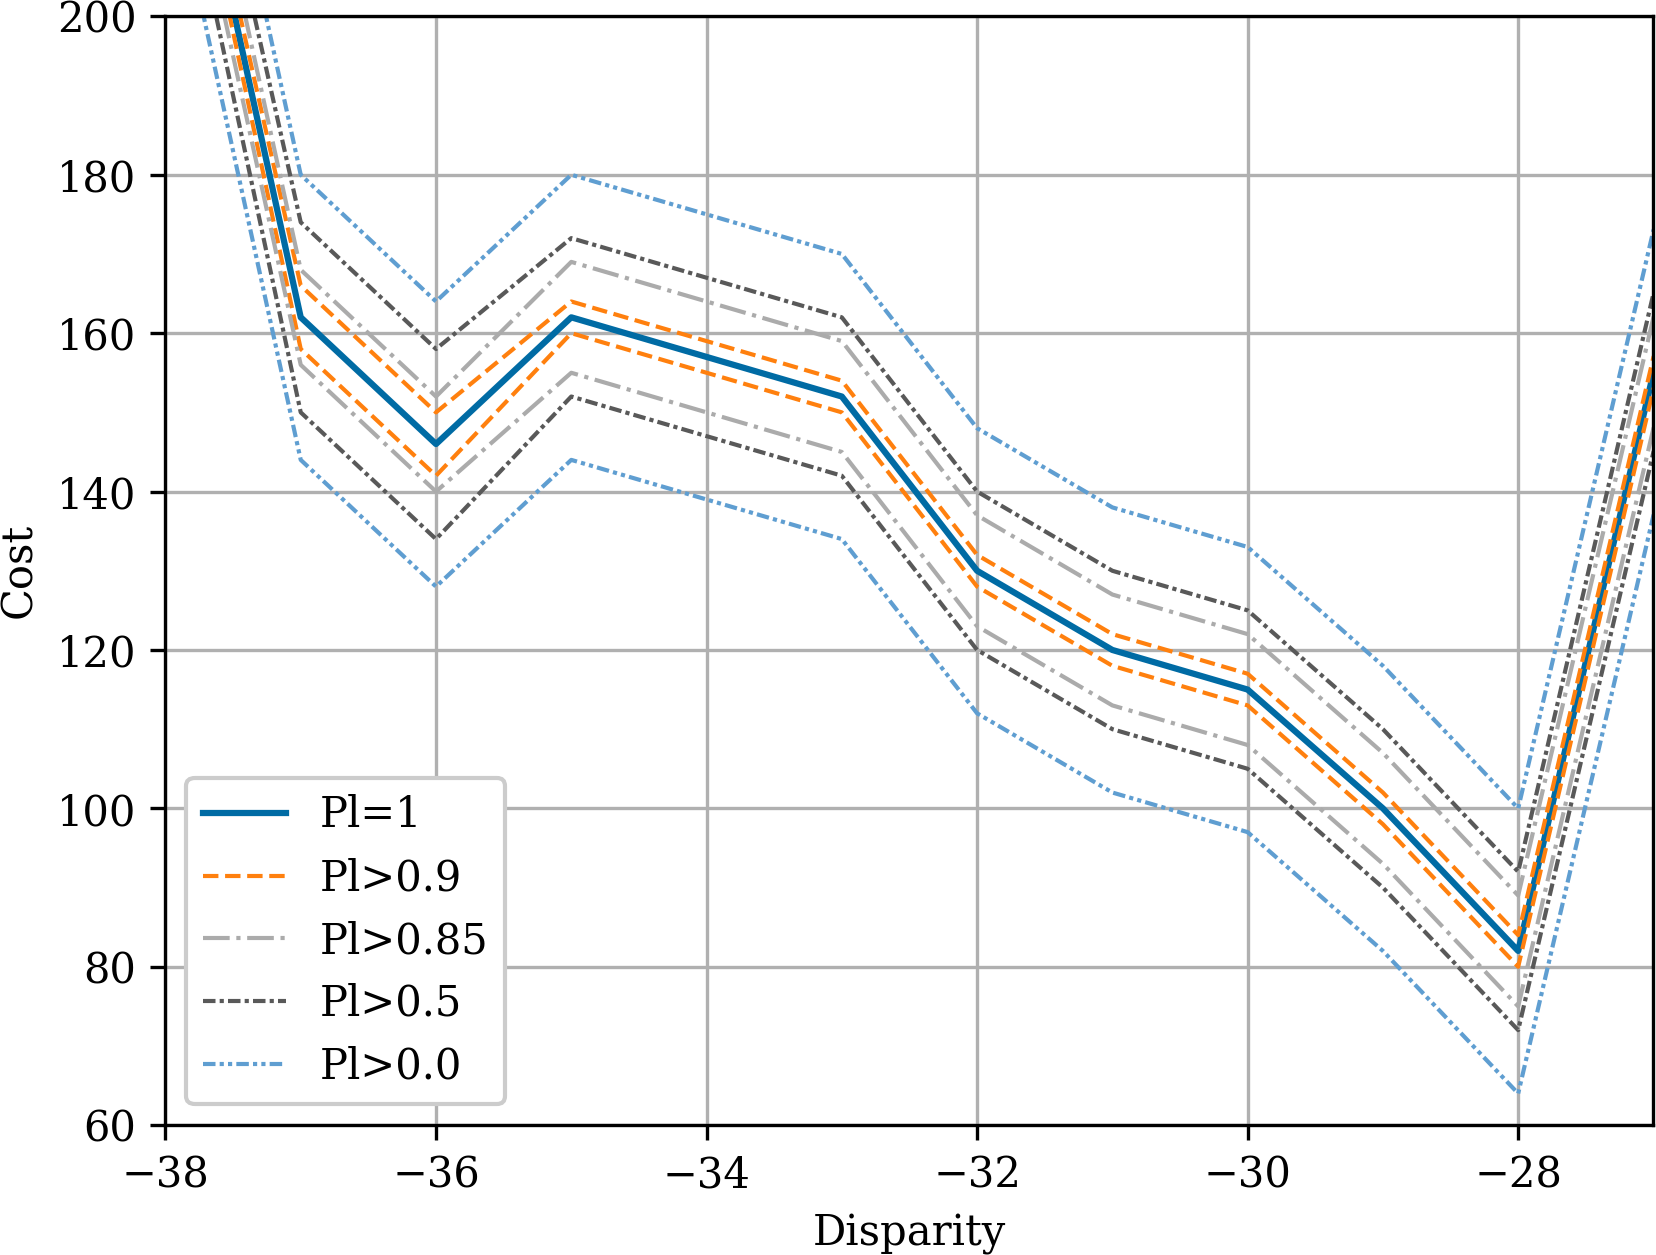
\includegraphics[width=\linewidth]{Images/Chap_4/bel_100_120_zoom.png}
        \caption{Detailed view of the rectangular section of \ref{fig:belief_gaussian}}
        \label{fig:belief_gaussian_zoom}
    \end{subfigure}
    \caption{Plausibility levels of a cost curve for the product copula $C_\Pi$ and the Gaussian copula $C_R$. The green vertical line represents the true disparity. Rectangular sections from the left figures are detailed on the right. From \cite{malinowski_uncertainty_2024}.}\commanue{j'ai pas l'impression que tu mentionnes à quel pixel ces courbes correspondent}
    \label{fig:belief_curves}
\end{figure}

A visualization of different plausibility levels of the $\SAD$ cost curve are presented in \Cref{fig:belief_curves}, computed with the product copula $C_\Pi$ and a Gaussian copula $C_R$. Both copula have the same support $\Pl>0$, and the same value for $\Pl=1$. Envelopes of the other plausibility levels are however different. \Cref{fig:belief_independence_zoom} and \Cref{fig:belief_gaussian_zoom} display the fact that the values covered by the plausibility levels vary with the copula used. Plausibility levels $0.85$ and $0.5$ are more concentrated around plausibility level $1$ in the case of the product copula than in the case of the Gaussian copula. Conversely, plausibility level $0.9$ is closer to plausibility level $1$ in the case of the Gaussian copula. This is due to the fact that the Gaussian copula $C_R$ is more co-monotone than the product copula given the correlation matrix $R$ described in \cref{eq:correlation}\commanue{là tu pointes sigma et pas R a priori c'est pas le bon label}.
\begin{remark}
    Both the Gaussian and the product copula have the same support. This is because when computing the joint mass of marginal focal sets, the copula is regular enough to assign a non-null mass to every focal set. This would not have been the case if we took a copula close to the lower or upper Fréchet-Hoeffding bound (the lower bound is not a copula for $n>2$). Indeed, those copulas are less regular, and can assign a null mass to joint events, as we saw in the case of probabilities in example \ref{ex:copulas} and more recently in example \ref{ex:propagated_probability}.
\end{remark}

\subsection{Estimating Propagated Credal Sets Using Monte Carlo Sampling}\label{sec:montecarlo}
In \Cref{chap:joining_credal_sets}, we defined $3$ methods for creating multivariate credal sets: $\M_{robust}$, $\M_{mass}$ and $\M_{agg}$. In the case where marginals were possibility distributions, we saw that the bounds of $\M_{agg}$ and $\M_{mass}$ were the same on Cartesian products, so we only considered $\M_{mass}$ in our application. In the previous sections, we propagated the uncertainty by using the approach from $\M_{mass}$. In this section, we will try to estimate the propagated uncertainty using $\M_{robust}$, and compare it to previous results so as to evaluate whether or not we can use $\M_{mass}$ to outer/inner approximate $\M_{robust}$.

We remind here some definitions and results regarding $\M_{robust}$. $\M_{robust}$ is the convex hull $CH$ of the set of every CDF from $n$ marginal credal sets $\M_i$ (in our case $n=18$, one per pixel involved in the $\SAD$ computation) joined with a copula $C$ (\cref{eq:robust_set}):
\begin{align*}
    \M_{robust} = CH(\{F=C(F_1 \enum F_n),~F_i\in\M_i \})
\end{align*}
We can estimate $\M_{robust}$ using Monte Carlo samplings: we first generate marginal probability distributions $F_1\enum F_n$ belonging in their respective marginal credal sets \cite{troffaes_note_2017}, then sample from the joint CDF $F$\commanue{Donc là c'est la version résumé et ensuite tu détailles donc il faudra mettre un petit mot de tarnsition. Je sais pas To do so ou IN detail ou un autre choix}. For each of the $18$ considered pixels, we sample a marginal CDF $F_i$ belonging to the credal set defined in \cref{eq:pixel_possibility}. The sampling from credal sets is not random: we generate probability distributions in such a way that for each marginal event $A$, the probability range $[\Nec(A), \Pi(A)]$ is sampled uniformly. With this method, we get a good coverage of each marginal credal set. We are also insuring that lower and upper bounds on events are all reached at least once, in order to include ``extreme'' distributions in our simulations. Once we have a CDF $F_i$ from each marginal CDF $F_i$, we can sample from the joint CDF using the method detailed in \Cref{sec:sampling_copula}. This yields a noised version of both left and right images, where the noised dependency is modeled by the provided copula, and its distribution is coherent with the possibility distributions from \cref{eq:pixel_possibility}. We can then compute a noised version of the cost volume from those images. For each cost curve, this provides a Monte Carlo samples of the $\SAD$ cost curves.

We compute $10\,000$ samples CDFs from each marginal credal set to construct the multivariate CDF. Each multivariate CDF is then itself sampled $10\,000$ times. The Central Limit Theorem states that $N$ Monte Carlo samples gives you an approximation with a precision of around $\frac{1}{\sqrt{n}}$\commanue{pourquoi le n est petit dans la formule ?} (it also depends on the standard deviation of the density you are estimating, but it is a good enough approximation), so $N=10\,000$ provides a satisfying precision for our application.  

In practice, we do not simulate a full noised pair of images at once, as it would require to sample from a copula of very large dimension (the number of pixels in both images). This is not realistically feasible, even thought it would ensure that each time a pixel is considered in the cost volume, the same noise samples are used. We instead generate noise samples for each row separately: noised values of pixels will not change during the evaluation of a cost curve for different disparities, or between the cost curves of pixels of the same row. However, their values might change between cost curves of pixels belonging to different rows. For instance, let's consider a pixel $p=(row,~col)\in I_L$ for which we computed a noised intensity $i_p$. We will use the same noised value $i_p$ of intensity when computing the $\SAD$ of every pixel $q=(row,~col')\in I_L$. But when computing the $\SAD$ of every pixel $q=(row-1,~col')\in I_L$, we will use a different Monte Carlo draw $i_p'$ for its intensity, which will stay the same for every pixel of row $row-1$. Because we draw a high number of Monte Carlo draws for each row, proceeding as such should not be noticeable. 

\begin{remark}
    As we construct the correlation matrices $R$ based on the segmentation of the left and right images, the cost curves presented in \Cref{fig:montecarlo_gauss_100_120,fig:montecarlo_gauss_200_150} mostly use a different copula for each disparity. Providing the values of those matrices would necessitate to represent around $60$ $18\times18$ correlation matrices, and is thus not provided here.
\end{remark}

\begin{figure}
    \centering
    \begin{subfigure}[t]{1\linewidth}
        \centering
        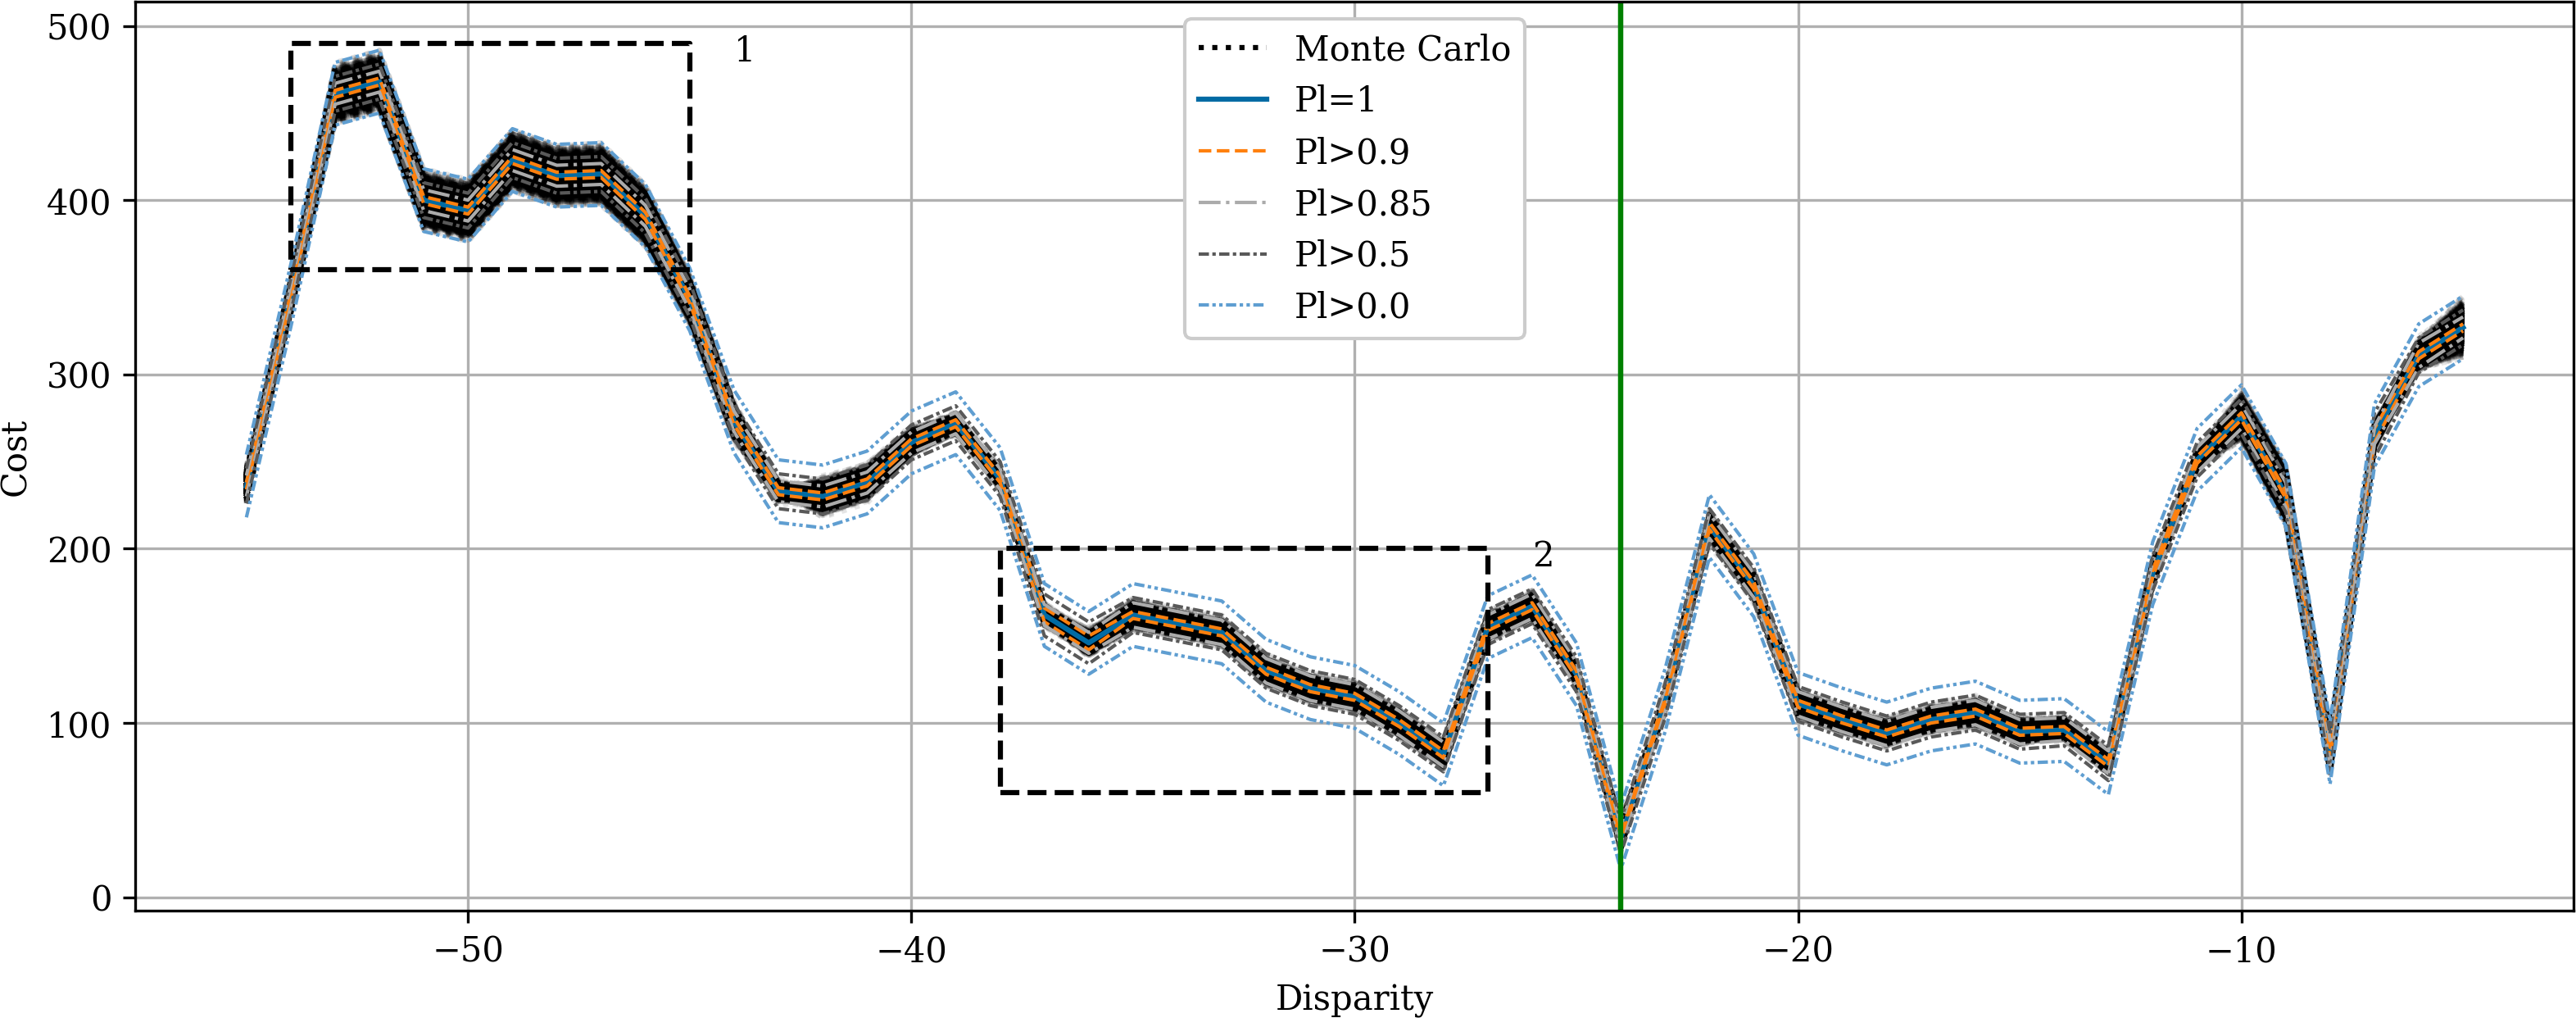
\includegraphics[width=\linewidth]{Images/Chap_4/cost_curve_100_120.png}
        \caption{Plausibility levels and Monte Carlo sampling using a Gaussian copula}
        \label{fig:montecarlo_gauss_100_120_large}
    \end{subfigure}\\
    \begin{subfigure}[t]{0.45\linewidth}
        \centering
        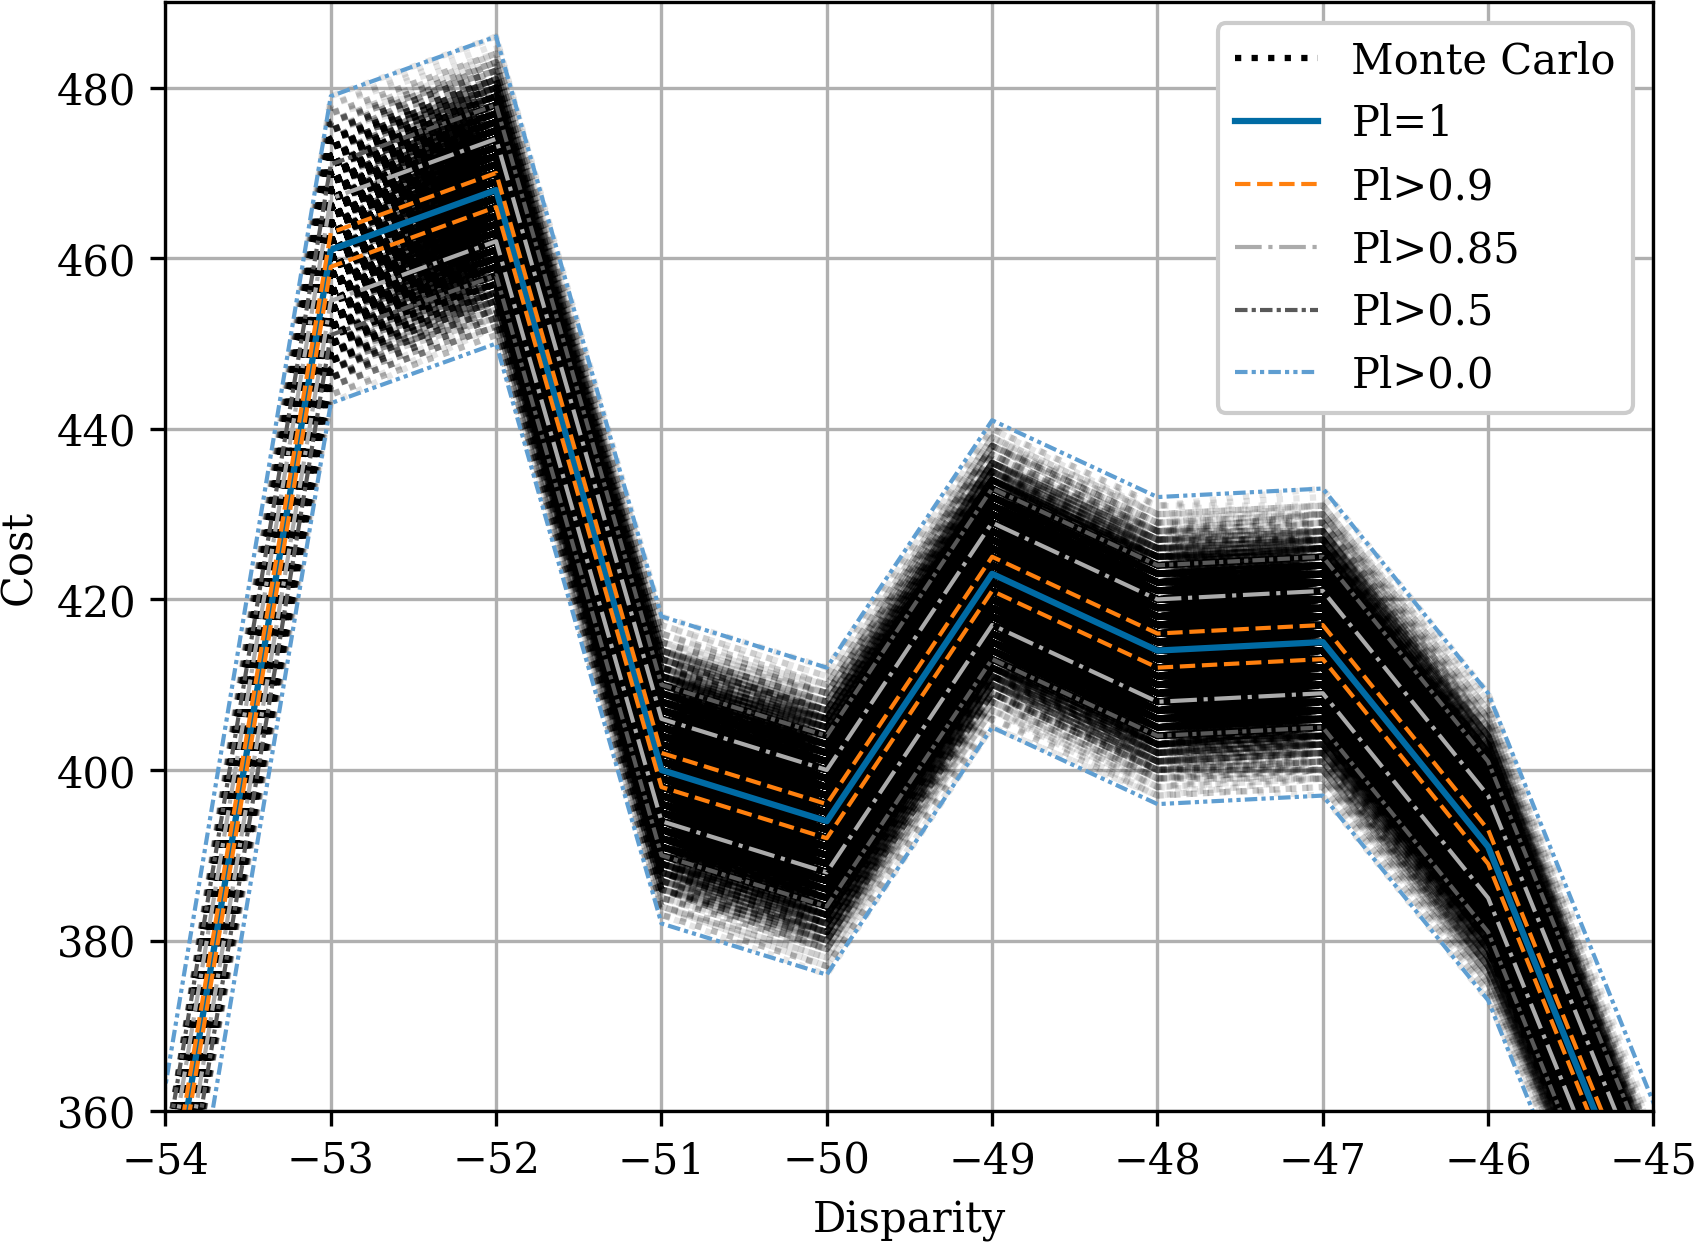
\includegraphics[width=\linewidth]{Images/Chap_4/cost_curve_100_120_zoom1.png}
        \caption{Zoom over the first rectangle}
        \label{fig:montecarlo_gauss_100_120_zoom1}
    \end{subfigure}\hfill
    \begin{subfigure}[t]{0.45\linewidth}
        \centering
        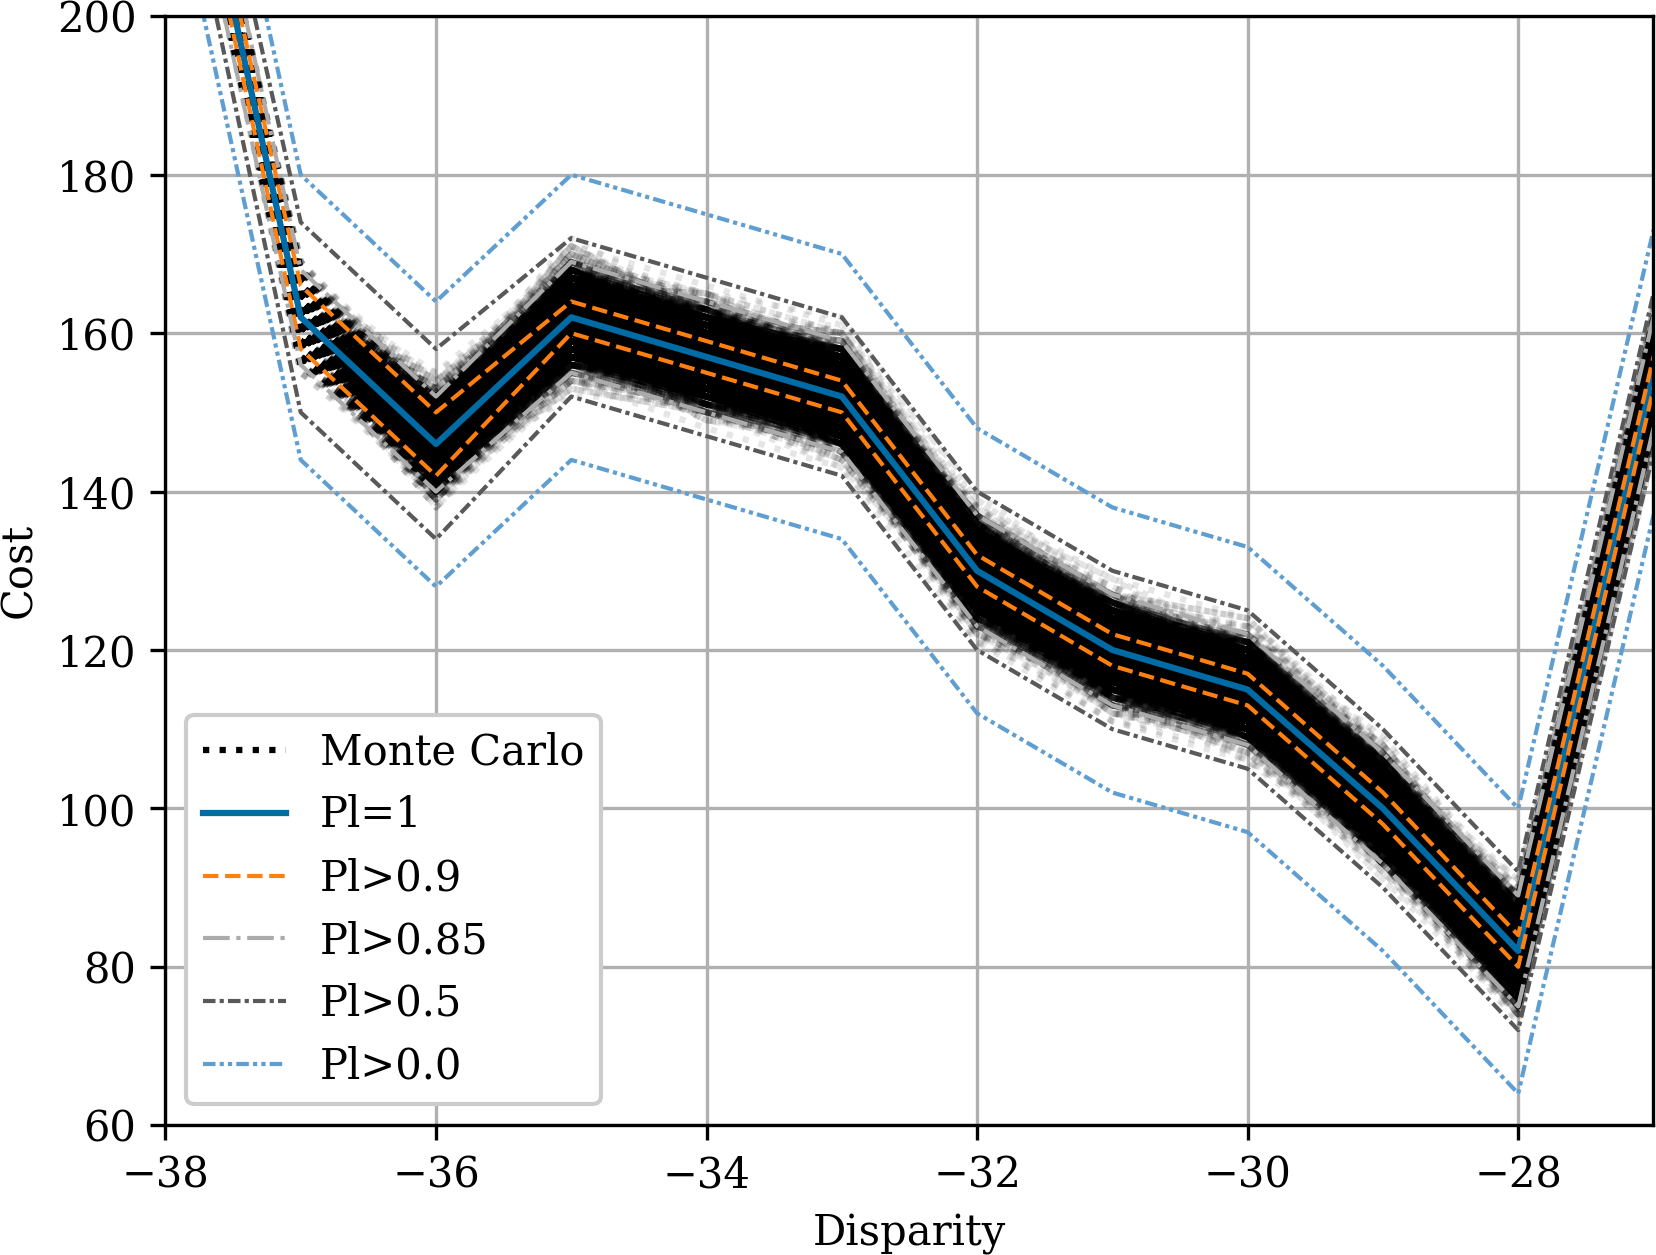
\includegraphics[width=\linewidth]{Images/Chap_4/cost_curve_100_120_zoom2.png}
        \caption{Zoom over the second rectangle}
        \label{fig:montecarlo_gauss_100_120_zoom2}
    \end{subfigure}
    \caption{Plausibility levels and Monte Carlo sampling for a pixel of the left image. From \cite{malinowski_uncertainty_2024}.}
    \label{fig:montecarlo_gauss_100_120}
\end{figure}

\begin{figure}
    \centering
    \begin{subfigure}[t]{\linewidth}
        \centering
        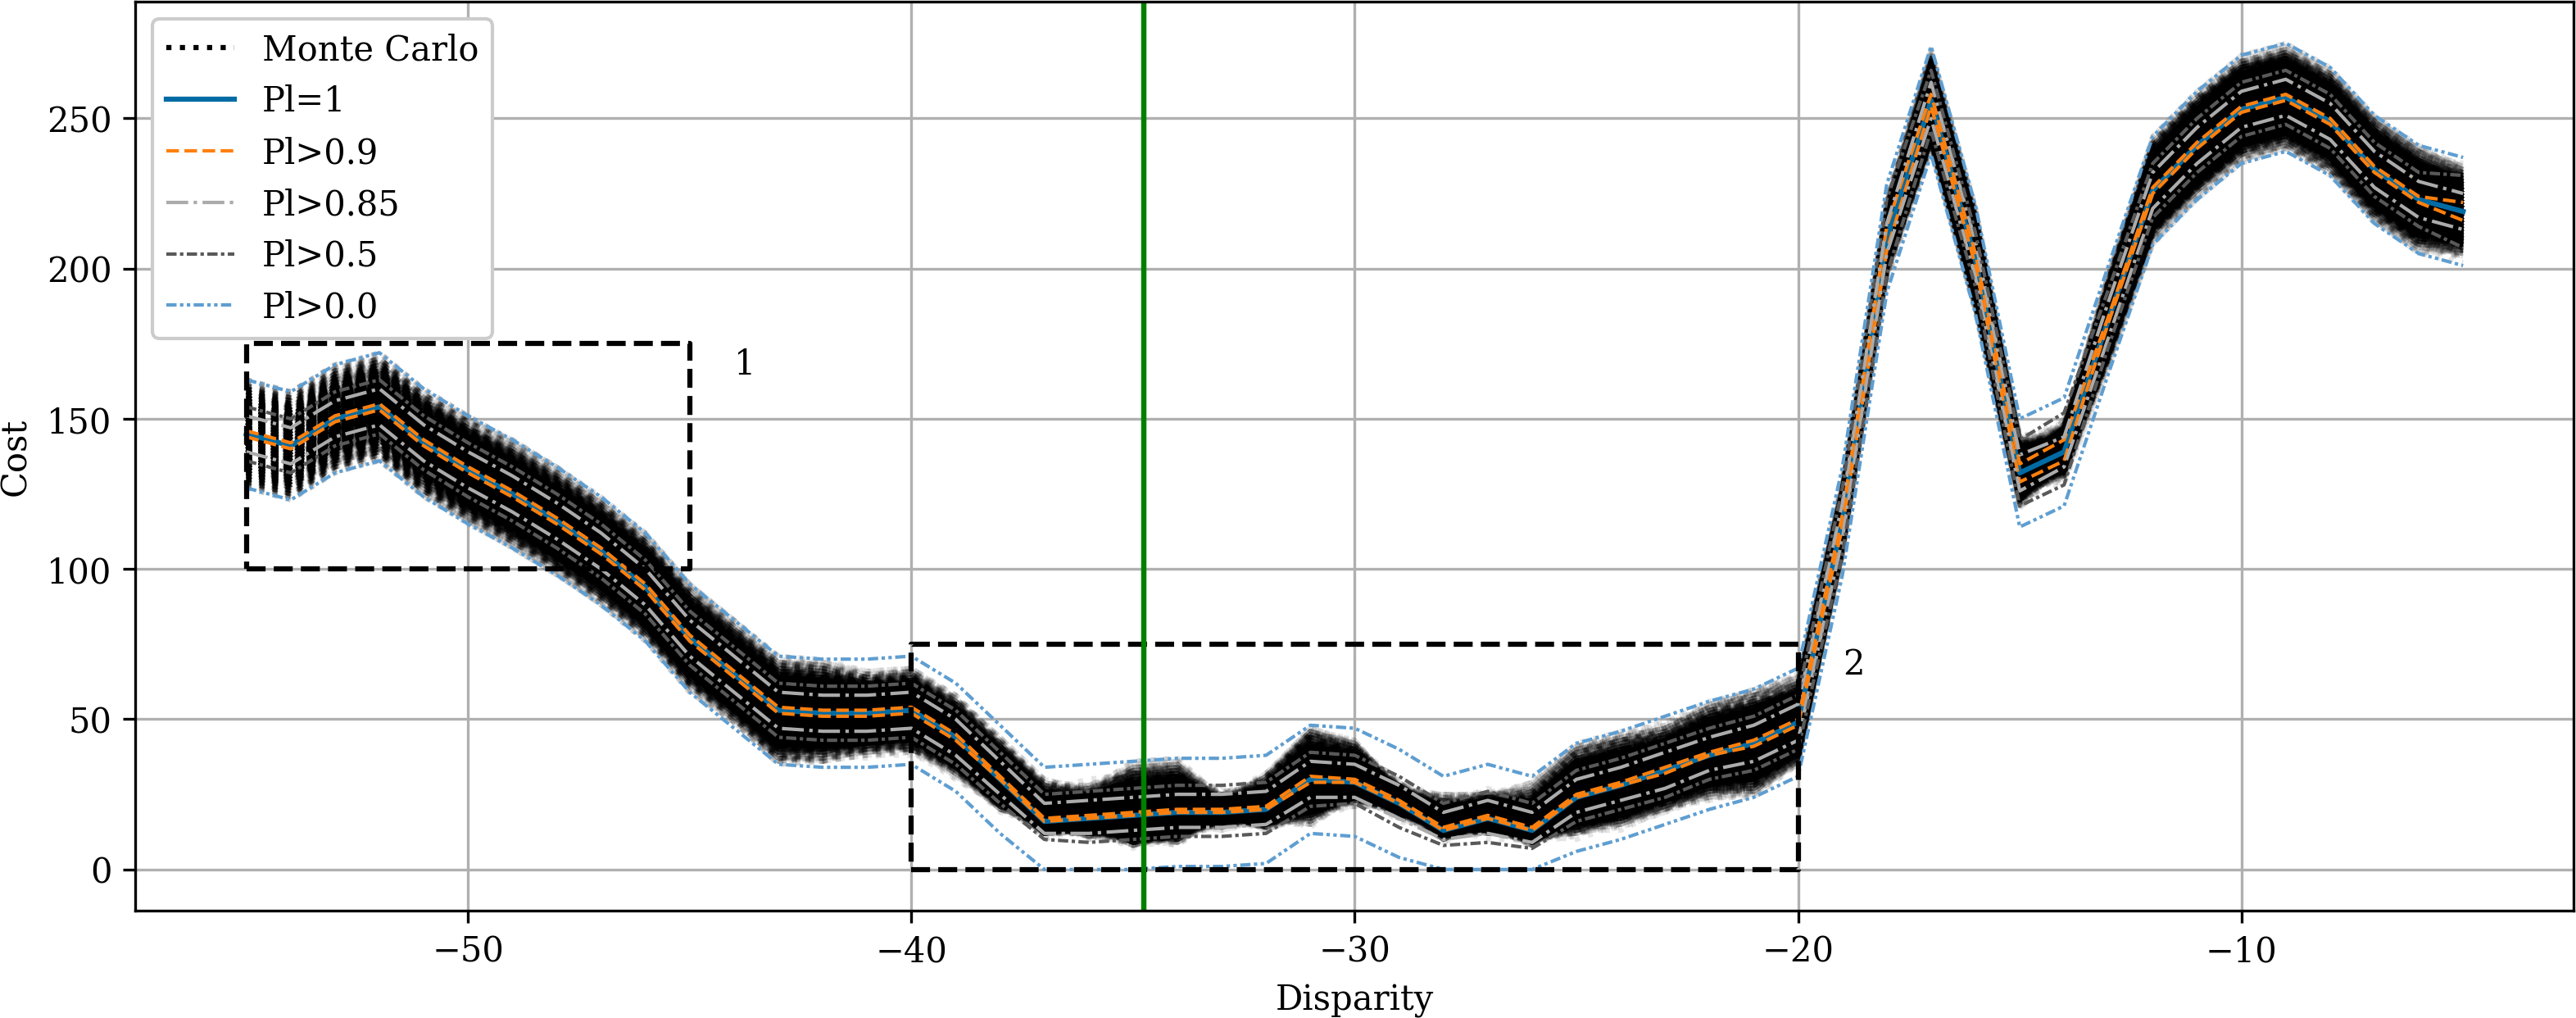
\includegraphics[width=\linewidth]{Images/Chap_4/cost_curve_200_150.png}
        \caption{Plausibility levels and Monte Carlo sampling using a Gaussian copula}
        \label{fig:montecarlo_gauss_200_150_large}
    \end{subfigure}\\
    \begin{subfigure}[t]{0.45\linewidth}
        \centering
        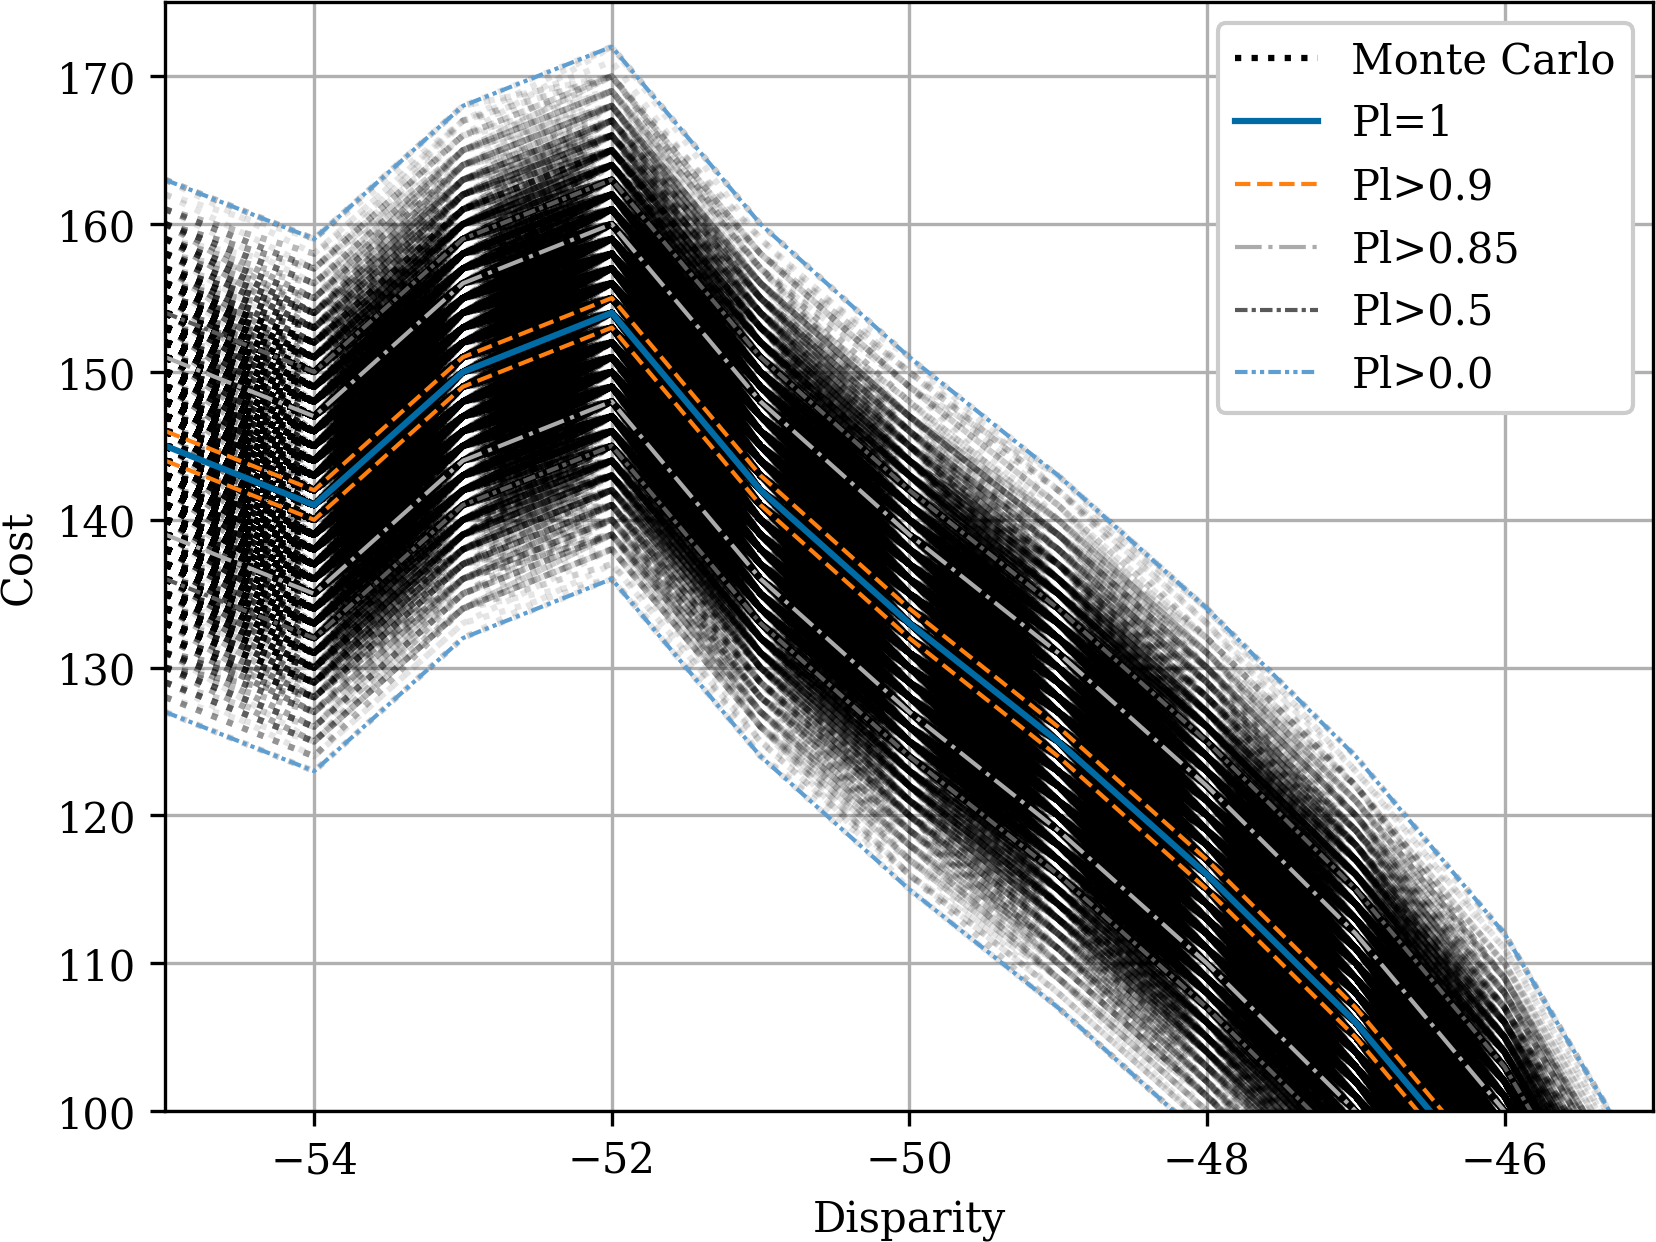
\includegraphics[width=\linewidth]{Images/Chap_4/cost_curve_200_150_zoom1.png}
        \caption{Zoom over the first rectangle}
        \label{fig:montecarlo_gauss_200_150_zoom1}
    \end{subfigure}
    \hfill
    \begin{subfigure}[t]{0.45\linewidth}
        \centering
        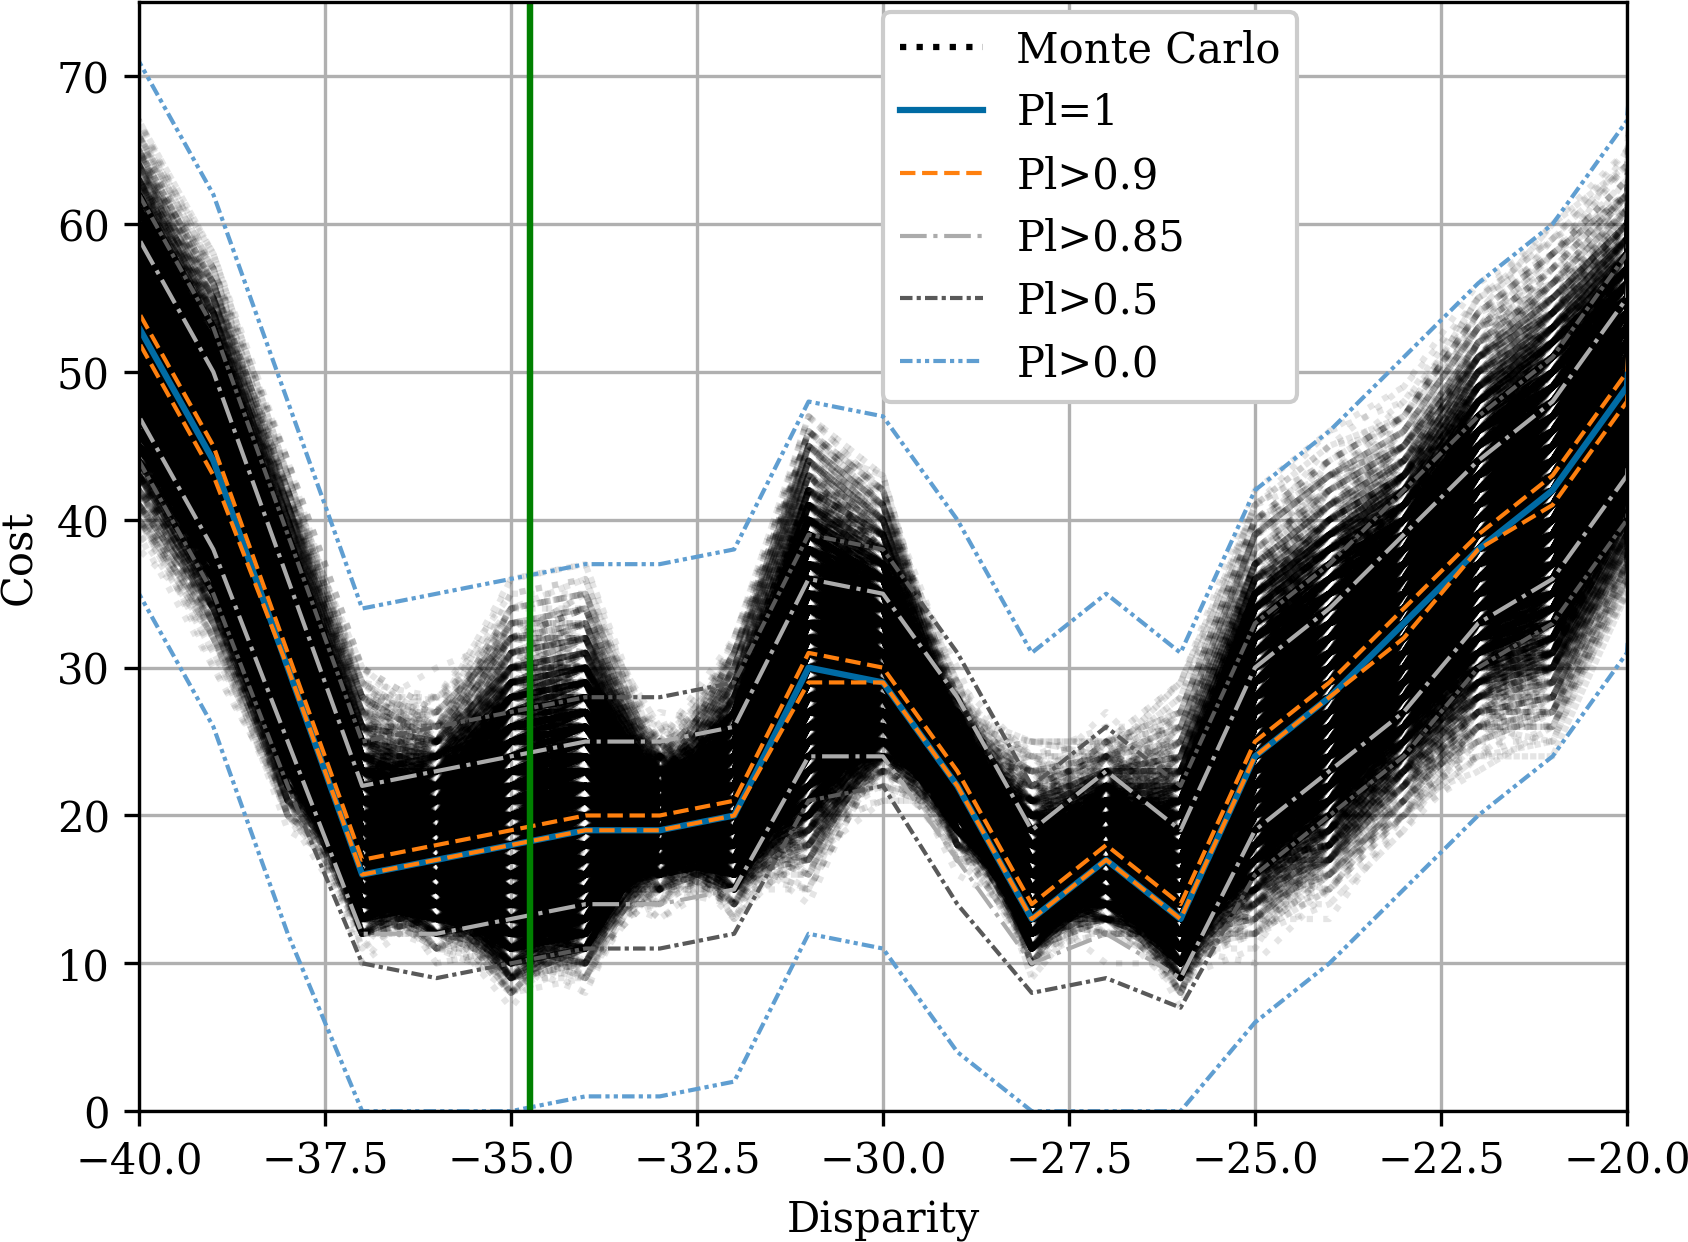
\includegraphics[width=\linewidth]{Images/Chap_4/cost_curve_200_150_zoom2.png}
        \caption{Zoom over the second rectangle}
        \label{fig:montecarlo_gauss_200_150_zoom2}
    \end{subfigure}
    \caption{Plausibility levels and Monte Carlo sampling for a pixel of the left image.  From \cite{malinowski_uncertainty_2024}.}
    \label{fig:montecarlo_gauss_200_150}
\end{figure}

Monte Carlo draws using the Gaussian copula and marginals credal sets of \cref{eq:pixel_possibility} are plotted in \Cref{fig:montecarlo_gauss_100_120,fig:montecarlo_gauss_200_150}. They respectively correspond to the cost curves of pixel located at positions $(100,~120)$ and $(200,~150)$ on the left image\commanue{alors les deux figures ont actuellement la même légende tu pourrais préciser la localisation du pixel dans la légende et cerise sur le gateau tu pourrais afficher l'image des cônes ou dire à quoi correspondent les deux pixels choisis car perso moi je ne sais pas à quel endroit ça correspond.}. Plausibility levels from \Cref{fig:belief_curves}\commanue{est-ce qu'il ne faudrait pas dire que tu affiches les plausibility levels de ces pixels calculés comme décrit pécédemment car dans la figure 4.4 tu ne considères qu'un seul pixel} also appear for comparison. The support envelopes from plausibility levels $\Pl>0$ correctly contain all Monte Carlo samplings for all considered copulas. We can observe in \Cref{fig:montecarlo_gauss_200_150_zoom2} that plausibility levels sometimes fail to correctly grasp the fluctuations of the dispersion of the samples, even though they correctly contain Monte Carlo samples. More specifically, Monte Carlo draws are first dense around disparity $-37$, then seem to spread around $-35$, and finally regather around disparity $-32$. The plausibility envelopes are more regular in this disparity range. This illustrates the fact the ``true'' point-wise credal $\M_{robust}$ set described in \Cref{sec:robust_method} is different from the joint credal set $\M_{mass}$ from \Cref{sec:joint_mass}. 

Although some differences persist between those sets, \Cref{fig:montecarlo_gauss_100_120_zoom2,fig:montecarlo_gauss_200_150_zoom2} suggest that the point-wise credal set $\M_{robust}$ can be outer approximated by $\M_{mass}$ in our applications. To quantify this observation, we can compute the proportion of Monte Carlo samples contained inside the plausibility envelopes for different plausibility levels $\gamma$:
\begin{align}
    \textrm{coverage}_\gamma = \frac{\#\{\textrm{ Monte Carlo samples }\in[\underline{I}_\gamma,~\overline{I}_\gamma]\}}{\#\{\textrm{ Monte Carlo samples }\}}
\end{align}
The coverage for the considered values of $\gamma$ are presented in \Cref{tab:Coverage}, where the first two rows represent the coverage of \Cref{fig:montecarlo_gauss_100_120,fig:montecarlo_gauss_200_150}. The global coverage over the whole left image is presented in the last row of the table. The coverage is always $100\%$ for $\gamma=0$, which shows that every sample is contained inside the support envelopes and that $\M_{robust}$ seems to be a subset of $\M_{mass}$. On the other hand, plausibility level $\gamma=0.5$ contain most Monte Carlo samples which means that the bounds could be significantly reduced while still being a good estimation of $\M_{robust}$. Finally, the variation of the coverage for plausibility levels $0.85$ and $0.9$ translates the previous observation that $\M_{mass}$ does not capture the variations of $\M_{robust}$ bounds and that those two set can substantially differ. Having estimated the uncertainty of the cost volume, we will see in the following section how we can leverage the upper and lower bounds for different plausibility levels to improve the disparity map derived from the cost volume.  

\begin{table}[ht]
\centering
\begin{tabular}{|c|c|c|c|c|}
\hline
\rowcolor[HTML]{C0C0C0}
$p=(row,col)$ & $\gamma=0.9$  & $\gamma=0.85$ & $\gamma=0.5$  & $\gamma=0$   \\ \hline
\cellcolor[HTML]{C0C0C0}$(100,~120)$     & $64,5\%$ & $94,5\%$ & $99,0\%$ & $100\%$ \\ \hline
\cellcolor[HTML]{C0C0C0}$(200,~150)$     & $30,0\%$ & $82,6\%$ & $95,2\%$ & $100\%$ \\ \hline
\cellcolor[HTML]{C0C0C0}Global        & $41,1\%$ & $87,6\%$ & $96,8\%$ & $100\%$ \\ \hline
\end{tabular}
\caption{Average coverage for various plausibility levels $\gamma$ and for different pixels $p$ of the left image.}\label{tab:Coverage}
\end{table}

\subsection{Leveraging Confidence Envelopes for Potential Improvements}\label{sec:sad_improvements}

Knowing the uncertainty, represented as confidence envelopes in our case, can provide valuable insights into potential matches. This section outlines different observations suggesting that incorporating this information can enhance the performance of stereo-matching algorithms.

From the cost volume $C_V$, we usually apply a \textit{winner-takes-all} strategy to compute a disparity prediction. Given a pixel $(row, ~col)$, the predicted disparity $\tilde{d}$ is defined as:
\begin{align}\label{eq:winner_takes_all}
    \tilde{d}(row, ~col) = \argmin_{d}C_V(row, ~col, ~d)
\end{align}
A common metric for evaluating stereo algorithm performance is the proportion of pixels for which the absolute difference between the true disparity $d_{true}$ and the predicted disparity $\tilde{d}$ is less than one pixel. The score \( s \) is defined as:
\begin{equation}\label{eq:score_d1}
    s = \frac{\#\{(row, col) \text{ such that } |d_{\mathrm{true}}(row, col) - \tilde{d}(row, col)| < 1\}}{\#\{(row, col)\}}\,.
\end{equation}
This metric is used as we usually only consider integer disparities (otherwise we need to upsample the stereo images\commanue{oui alors là c'est un peu un raccourci dans le remarque, vu ton pipeline (pas de raffinement) tu es sur des disparités entières. Mais la métrique elle est valable sur ce qu'on veut.}) but the ground truth disparity can be any real number in the disparity range\commanue{bah tu peux utiliser cette métrique avec n'importe quelle valeur de seuil. Là question est de savoir quelle est la précision de ta VT. Bref je comprends pas trop la phrase.}. We thus consider a disparity to be ``correct'' if it is less than one pixel away from the true disparity.

Having computed envelopes $\underline{I}_\gamma$, $\overline{I}_\gamma$ on the cost volume for different plausibility levels $\gamma$, the cost curve is not unique anymore, and we can instead consider all cost curves $C_{\underline{I}_\gamma,\overline{I}_\gamma}$ contained within the plausibility envelopes. Instead of a single predicted disparity, we can now compute the set of all potential disparities, defined as the set of predicted disparities from every cost curve contained in the plausibility envelopes. Given a pixel $(row, col)$, a confidence level $\gamma \in [0, 1]$, and plausibility envelopes $\underline{I}_\gamma(row, ~col, ~d)$, $\overline{I}_\gamma(row, ~col, ~d)$, the set of potential disparities $D_\gamma^{row, col}$ is defined as\commanue{Il y a un signe $\leqslant$ au milieu d'un intervalle}:
\begin{align}
    D_\gamma^{row, col} = \{d \mid& d=\argmin_\delta C_{\underline{I}_\gamma,\overline{I}_\gamma}(row,~col,~\delta),\\
    &\forall C_{\underline{I}_\gamma,\overline{I}_\gamma}(row, ~col, ~\delta)\in[\underline{I}_\gamma(row, ~col, ~\delta)\leqslant \overline{I}_\gamma(row, ~col, ~\delta)]\}\nonumber
\end{align}
There is actually a simpler way of defining and computing $D_\gamma$, which is to notice that a disparity can be the minimum of a cost curve $C_{\underline{I}_\gamma,\overline{I}_\gamma}$ if and only if the lower bound $\underline{I}_\gamma$ for this disparity is less than every upper envelope $\overline{I}_\gamma$\commanue{je comprends pas le terme every upper enveloppe. Tu fixes gamma et donc tu regardes qu'une seule enveloppe et tu t'assures que tu sois en dessous du min de la borne sup, ou alors j'ai rien compris}:
\begin{equation}
    D_\gamma^{row, col} = \{d \mid \underline{I}_\gamma(row, ~col, ~d) \leq \min_\delta\overline{I}_\gamma(row, col, \delta)\}
\end{equation}
\Cref{fig:potential_disparities} provides a schematic example of $D_\gamma(row, col)$.
\begin{figure}[ht]
    \centering
    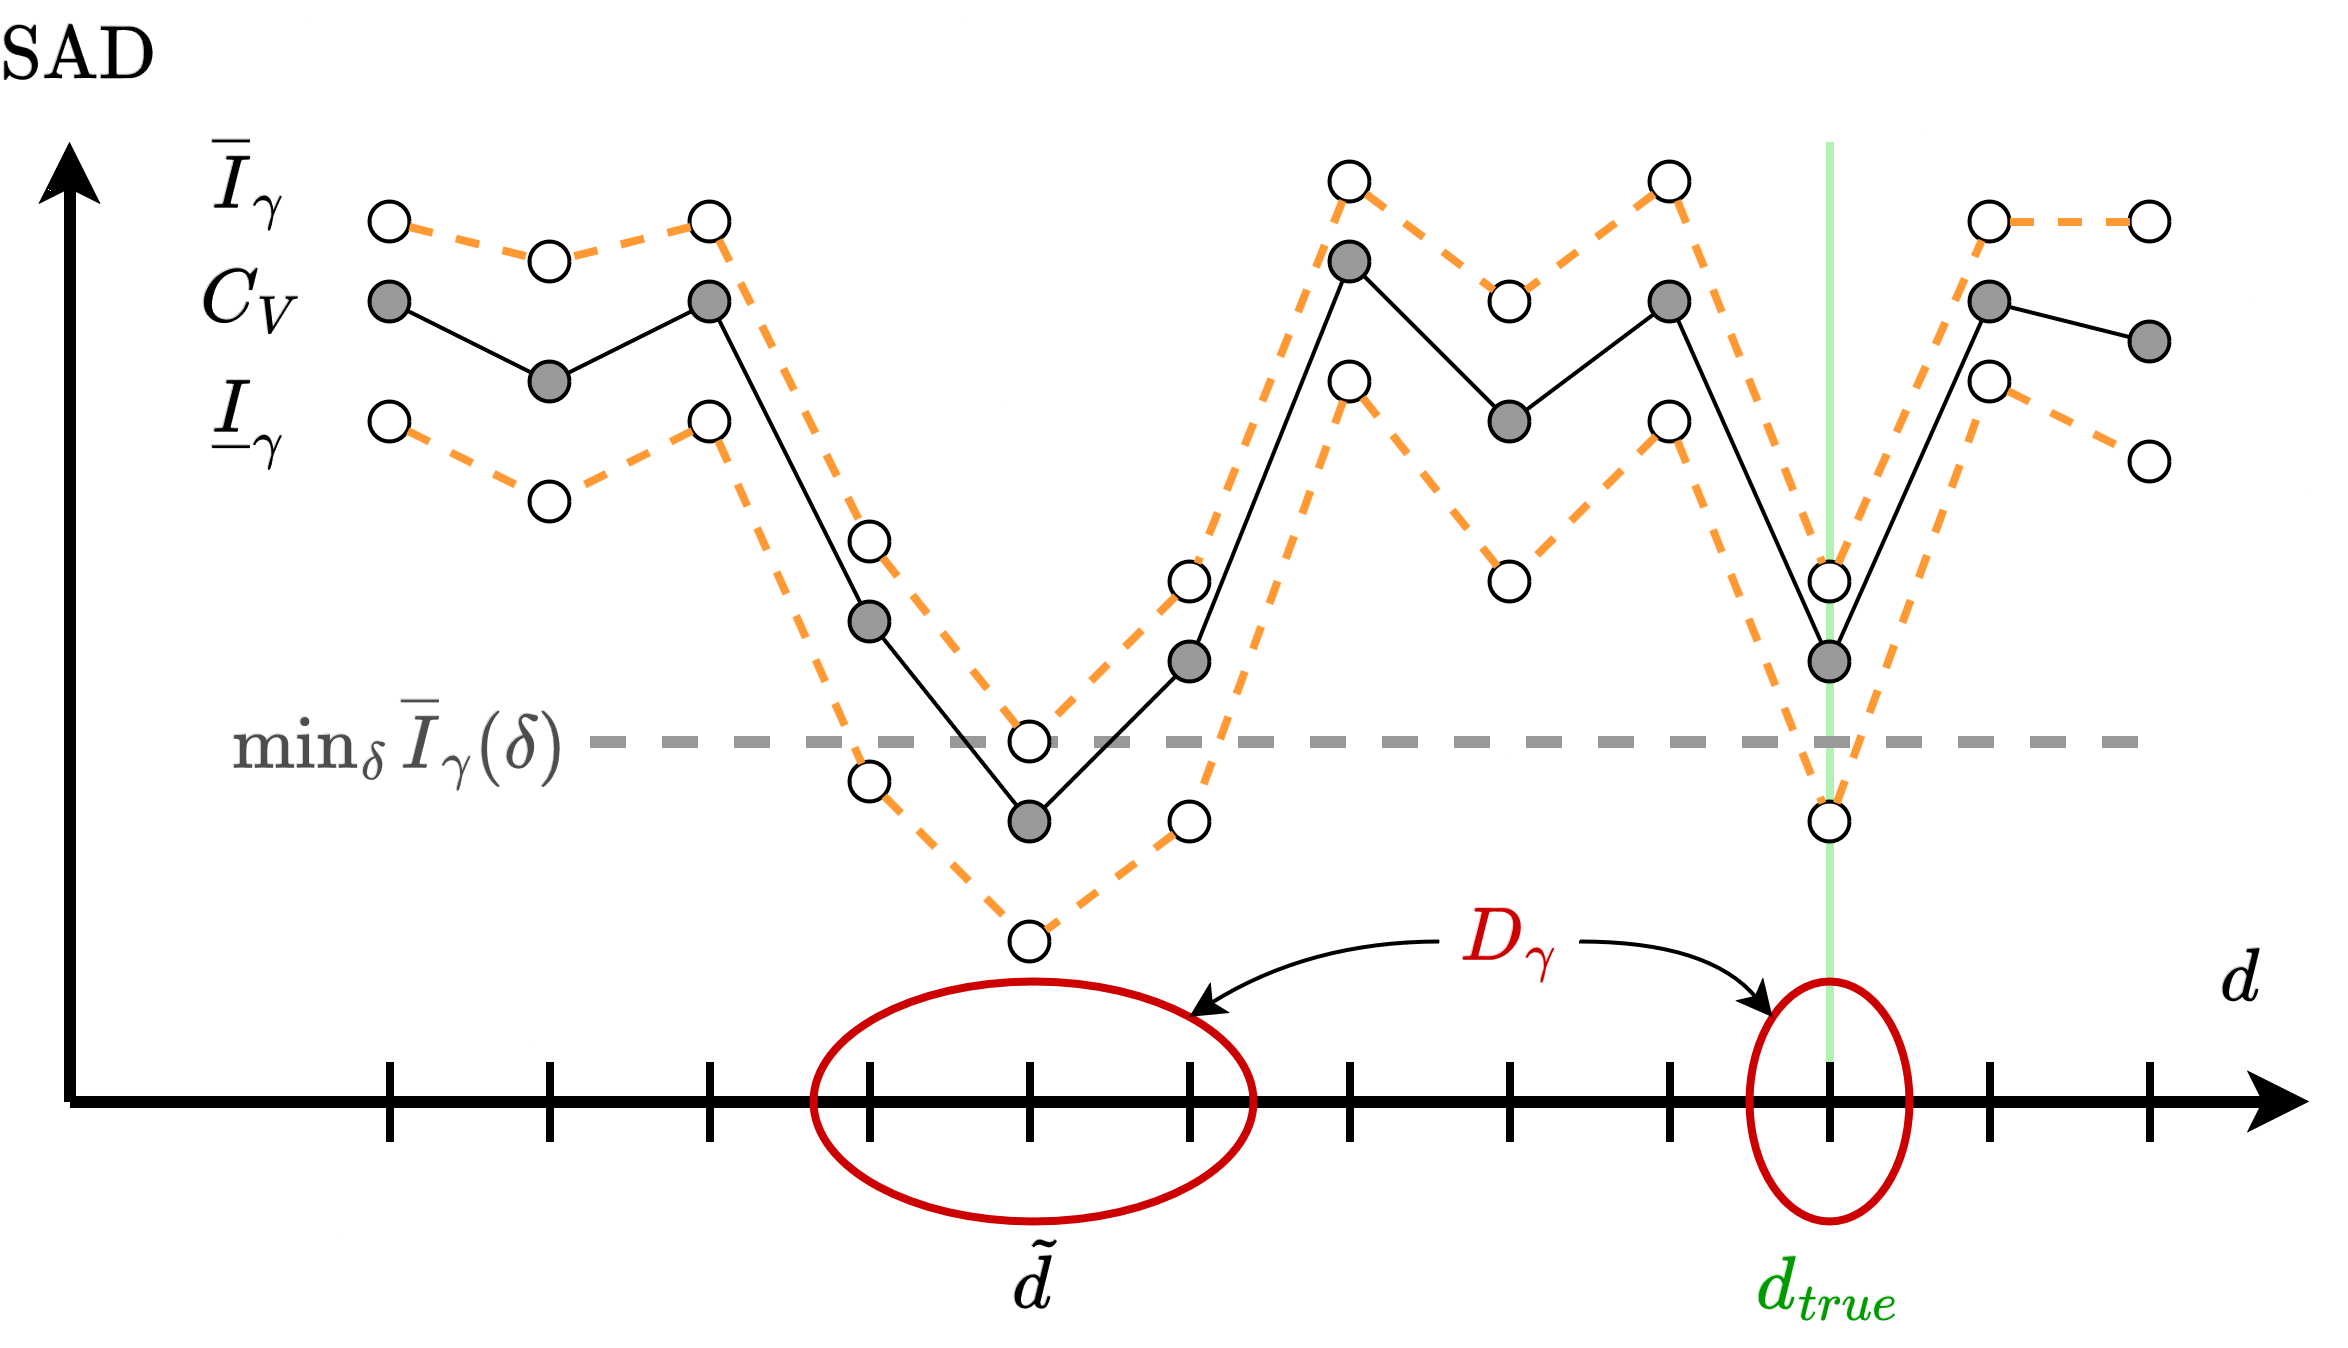
\includegraphics[width=\linewidth]{Images/Chap_4/Potentiel_disparities.png}
    \caption{Example of a set of potential disparities $D_\gamma$. The minimum of the upper envelope $\min\overline{I}_\gamma$ in dashed gray line. The vertical green line represents the true disparity.}
    \label{fig:potential_disparities}
\end{figure}

When the cost volume is considered without its uncertainty, many disparities are not correctly estimated by \cref{eq:winner_takes_all}. We thus want to quantify the potential score improvements contained in the set of potential disparities $D_\gamma$. To do so, we consider that $D_\gamma$ is a potential improvements if it contains the true disparity $d_{true}$. From this we can compute the proportion of potential improvements $s_\gamma^{\text{opt}}$ over the whole image, and compare it to the score $s$ computed without uncertainty from \cref{eq:score_d1}. The proportion of potential improvements, or optimal score, \( s_\gamma^{\text{opt}} \) achievable using the set of possible disparities is computed as follows\commanue{là ça fait redite donc introduis et définis ton score optimal et ensuite tu dis que tu le compares. Là tu introduis, dis que tu vas le comparer et ensuite tu le définis. C'est le tiercé dans le désordre.}:
\begin{equation}\label{eq:optimal_score}
    s_\gamma^{\text{opt}} = \frac{\#\{(row, col) \mid \min_{d \in D_\gamma^{row, col}} |d_{\mathrm{true}}(row, col) - d| < 1\}}{\#\{(row, col)\}}
\end{equation}
In \Cref{fig:potential_disparities}, we can see that the predicted disparity $\tilde{d}$ is far away from the true disparity $d_{true}$, but the set of possible disparity $D_\gamma$ does indeed contain, the true disparity. This would have been counted as a potential improvement.

\begin{remark}
    \Cref{eq:optimal_score} defines the optimal score that \textit{could} have been obtained if we used an ideal cost volume contained in the envelopes. We do not provide a method for determining this ideal cost volume. In reality, even with a good strategy to leverage uncertainty information to obtain a better disparity map, the new score $s$ from \cref{eq:score_d1} would be lower than $s_\gamma^{\text{opt}}$.
\end{remark}

We define the potential gain as \( \Delta s_\gamma = s_\gamma^{\text{opt}} - s \). $\Delta s_\gamma$ measures the proportion of pixel that benefit from the method, \ie pixels $(row, ~col)$ verifying:
\begin{equation}
    |d_{\mathrm{true}}(row, ~col) - \tilde{d}(row, ~col)| \geq 1 \quad \text{and} \quad \min_{d \in D_\gamma^{row, col}} |d_{\mathrm{true}}(row, ~col) - d| < 1
\end{equation}

Examples of optimal scores and potential gains for various $\gamma$ values are provided in \Cref{tab:optimal_score}. We can see that while the potential gain for $\gamma = 0.9$ is low, it increases significantly for lower values of $\gamma$. The base score is around $53\%$, which is a relatively low score for dense matching, but that was expected as we are using the $\SAD$ without \acrshort{sgm} regularization or additional post processing. With $\gamma=0.85$, we could reach an optimal score of $67\%$, and using $\gamma=0.5$ or $\gamma=0$, the score could at best lie between $74\%$ and $82\%$. This is a quite significant improvement for a cost volume computed with the $\SAD$ cost function. For comparison, a $\SAD$ cost volume regularized with \acrshort{sgm} algorithm would have a score $s$ of $68\%$.

\Cref{fig:improvements} displays the spatial distribution of pixels that can benefit from this method. Pixels in occluded regions, \ie pixels only appearing in one of the two images, are highlighted in orange. As occluded pixels cannot be improved as no true disparity exists, we do not consider them when computing the different statistics introduced in this section. Pixels where potential improvement can occur appear in blue.

We can see that pixels with potential improvements are not randomly distributed. These pixels are typically found in homogeneous areas where multiple disparities have low matching costs, where the cost curves would be similar to the one represented in \Cref{fig:montecarlo_gauss_200_150_large}.
\comroman{Avec le recul ça aurait aussi été intéressant de voir si le nombre de disparité ou la dispersion de $D_\gamma$ pouvait être une mesure de confiance, calculer la courbe d'erreur comme dans le papier sur l'amb}\commanu{à mettre en perspective donc...}. 

\begin{table}[ht]
\centering
\begin{tabular}{|c|c|c|c|c|}
\hline
\rowcolor[HTML]{C0C0C0} 
$s=52.87\%$                                & $\gamma=0.9$ & $\gamma=0.85$ & $\gamma=0.5$ & $\gamma=0$ \\ \hline
\cellcolor[HTML]{C0C0C0}$s_\gamma^{opt}$   & $56.92\%$    & $66.99\%$     & $74.28\%$    & $81.75\%$  \\ \hline
\cellcolor[HTML]{C0C0C0}$\Delta s_\gamma$ & $4.05\%$     & $16.11\%$     & $21.41\%$    & $28.87\%$  \\ \hline
\end{tabular}
\caption{Optimal score and potential gain for different plausibility $\gamma$. The potential gain is computed with regards to the usual score $s=52,87\%$.}\label{tab:optimal_score}
\end{table}

\begin{figure}[ht]
    \centering
    \begin{subfigure}[t]{0.48\linewidth}
        \centering
        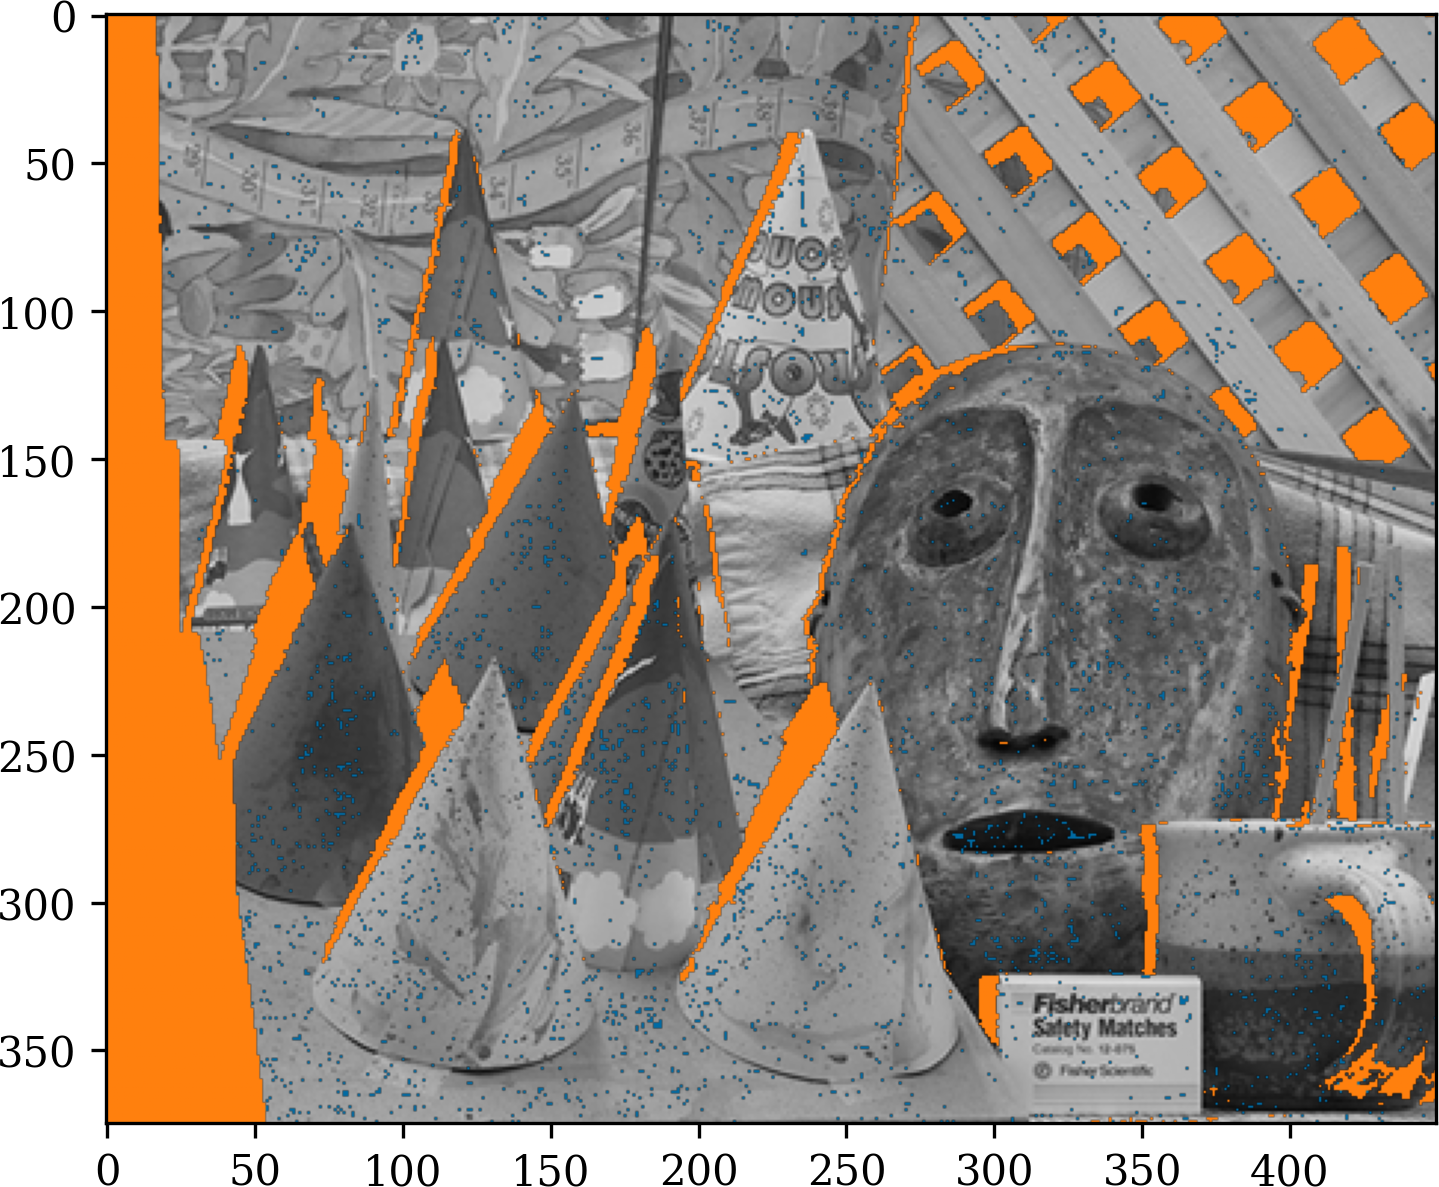
\includegraphics[width=\linewidth]{Images/Chap_4/Improvements_Pl=0.9.png}
        \caption{$\gamma=0.9,~\Delta s_\gamma=4.05\%$}
        \label{fig:improvements_a}
    \end{subfigure}
    \begin{subfigure}[t]{0.48\linewidth}
        \centering
        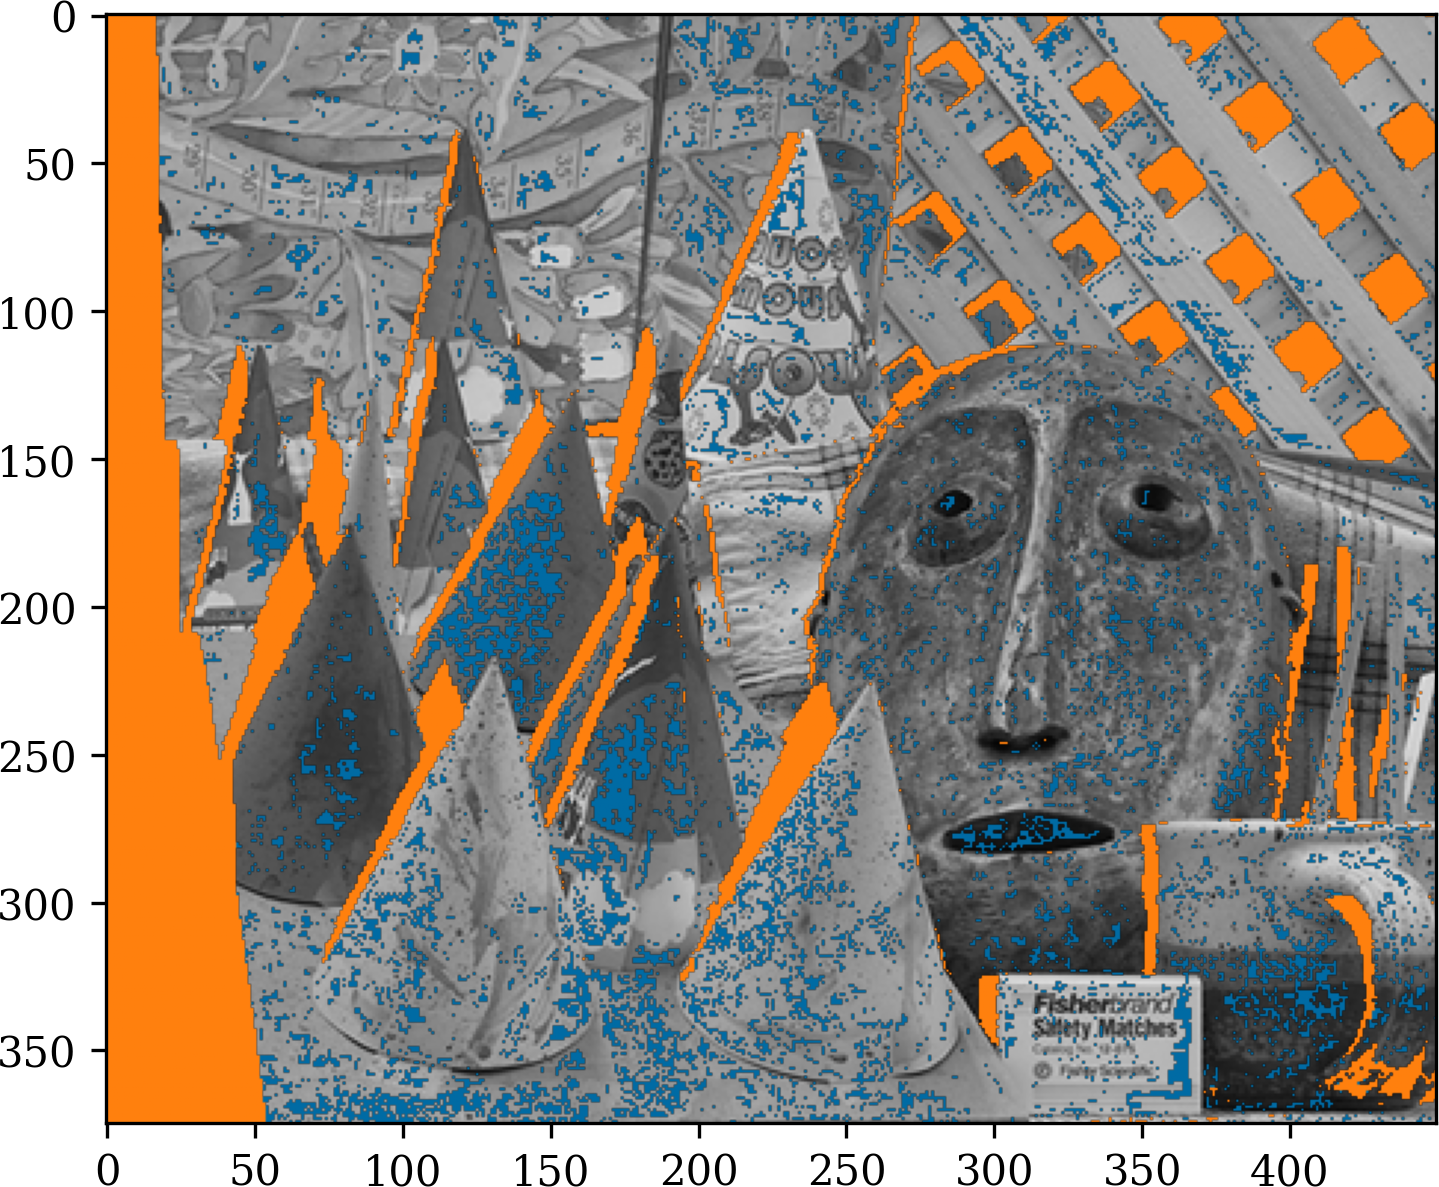
\includegraphics[width=\linewidth]{Images/Chap_4/Improvements_Pl=0.85.png}
        \caption{$\gamma=0.85,~\Delta s_\gamma=16.11\%$}
        \label{fig:improvements_b}
    \end{subfigure}\\
    \begin{subfigure}[t]{0.48\linewidth}
        \centering
        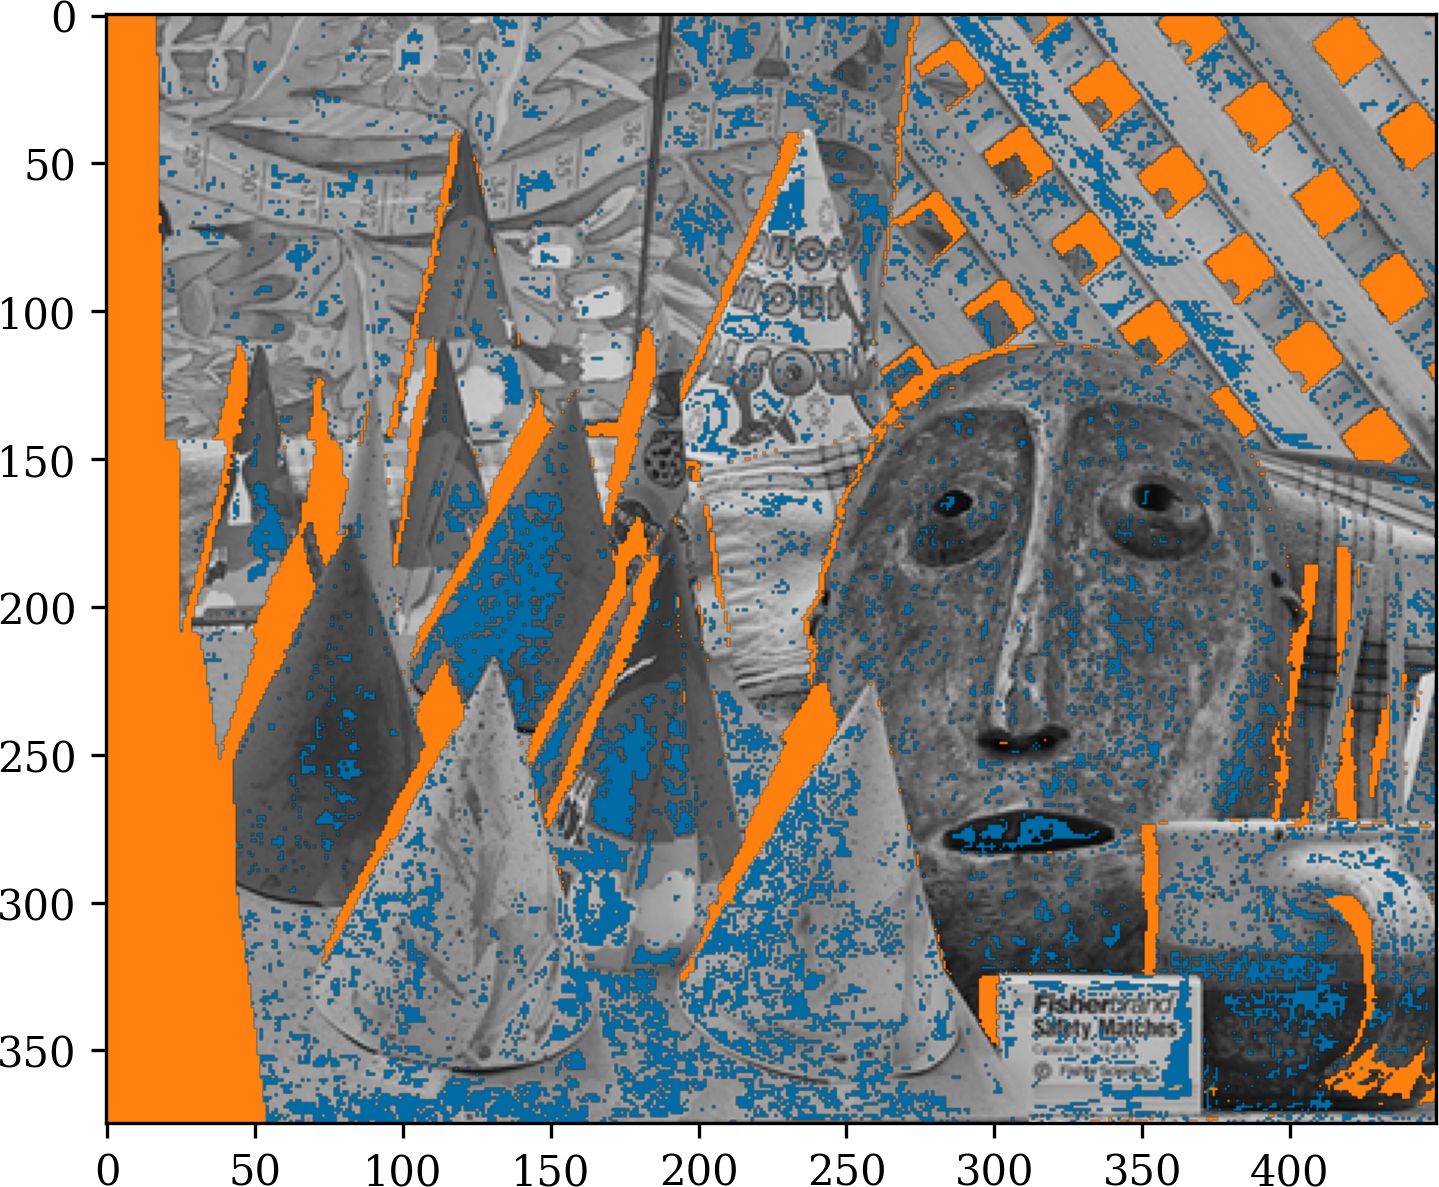
\includegraphics[width=\linewidth]{Images/Chap_4/Improvements_Pl=0.5.png}
        \caption{$\gamma=0.5,~\Delta s_\gamma=21.41\%$}
        \label{fig:improvements_c}
    \end{subfigure}
    \begin{subfigure}[t]{0.48\linewidth}
        \centering
        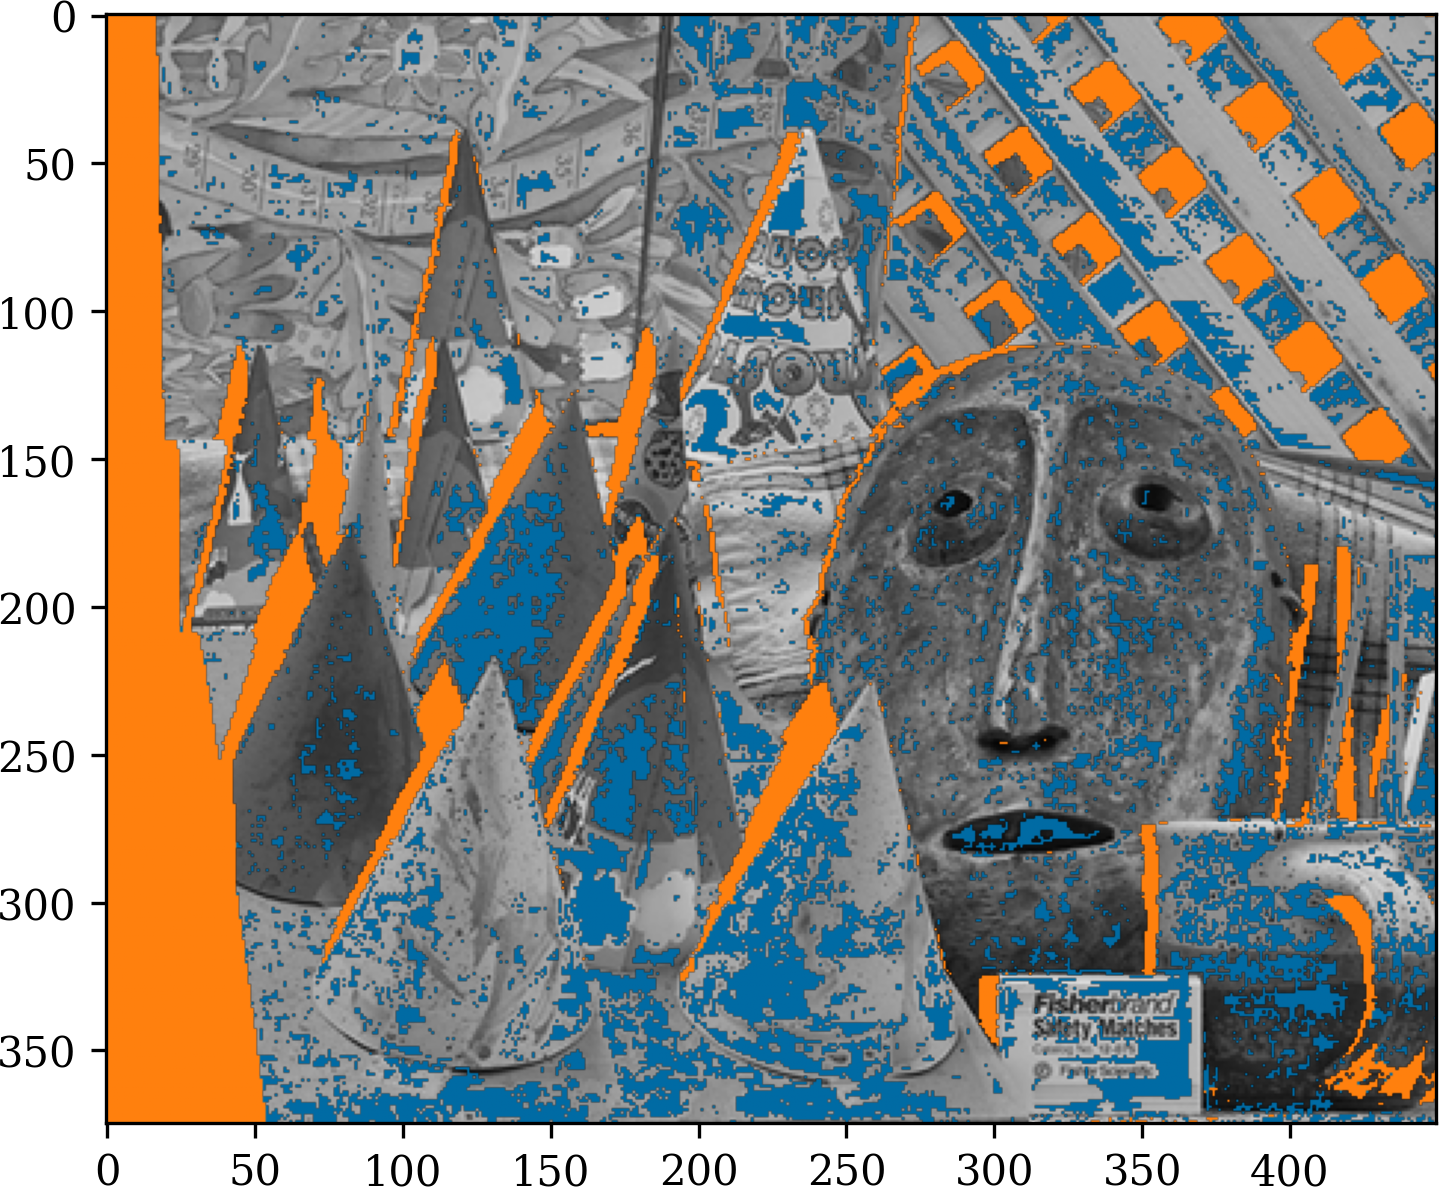
\includegraphics[width=\linewidth]{Images/Chap_4/Improvements_Pl=0.0.png}
        \caption{$\gamma=0,~\Delta s_\gamma=28.87\%$}
        \label{fig:improvements_d}
    \end{subfigure}
    \caption{Spatial disposition of potential improvements for different values of $\gamma$. Pixels with potential improvements appear in blue. Occluded pixels, for which a correct disparity does not exist, appear in orange. Grayscale left image is displayed on the background. From \cite{malinowski_uncertainty_2024}.}
    \label{fig:improvements}
\end{figure}

In this Chapter\commanue{oh mon dieu une conclusion, j'ai pas l'habitude, peut-être faire une section dédiée, c'est toi qui voit}, we modeled the uncertainty on stereo images and propagated it until the cost volume. We compared different methods from \Cref{chap:joining_credal_sets} for propagating the uncertainty, and evaluated the potential improvements unlocked by this uncertainty estimation. However, the stereo algorithm considered for computing the cost volume was intentionally simple to reduce the complexity of the problem. For the \acrshort{co3d} mission, different cost functions (CENSUS, MC-CNN) and \acrshort{sgm} regularization would instead be used. Furthermore, although the uncertainty on input images have an influence on the final uncertainty, the major part of the disparity map uncertainty comes from the processing uncertainty of the stereo algorithm itself. Quantifying and propagating this processing uncertainty will be thus be the subject of \Cref{chap:epistemic_uncertainty}.

\pagebreak
\blankpage